\documentclass[letterpaper, 10 pt, conference]{ieeeconf}  % Comment this line out if you need a4paper

%\documentclass[a4paper, 10pt, conference]{ieeeconf}      % Use this line for a4 paper

\IEEEoverridecommandlockouts                              % This command is only needed if 
                                                          % you want to use the \thanks command

\overrideIEEEmargins     
\let\proof\relax
\let\endproof\relax
\let\labelindent\relax
\usepackage{amssymb}
\usepackage{graphicx}
\usepackage[hidelinks]{hyperref}
\usepackage[ruled,resetcount,vlined]{algorithm2e}
\usepackage{commath}
\usepackage[font=small]{caption}
\usepackage{subcaption}
\usepackage{booktabs}
\usepackage{diagbox}
\usepackage{amsthm}
\usepackage{times} % assumes new font selection scheme installed
\usepackage{amsmath} % assumes amsmath package installed
% \usepackage{algorithm}
% \usepackage{algorithmic}
\usepackage{graphicx}
\usepackage{textcomp}
\usepackage[dvipsnames, table]{xcolor}
\usepackage{float}
\usepackage{wrapfig}
\usepackage{svg}
\usepackage{color, soul}
\usepackage[capitalize]{cleveref}
\usepackage[style=ieee, sorting=none,backend=biber, maxbibnames=2, minbibnames=1]{biblatex}
\addbibresource{bib.bib}
\usepackage{tikz,subcaption}
\usetikzlibrary{arrows.meta}
\usepackage{enumitem}
\usepackage{lipsum}


\newcommand{\ar}[1]{{\color{ForestGreen}AR:#1} }
\newcommand{\ap}[1]{{\color{purple}AP:#1} }
\newcommand{\gm}[1]{{\color{red}GM:#1} }
\newcommand{\rs}[1]{{\color{blue}RS:#1} }


\title{Moving On, Even When You're Broken: Fail-Active Trajectory Generation via Diffusion Policies Conditioned on Embodiment and Task \vspace{-10pt}}

% The \author macro works with any number of authors. There are two
% commands used to separate the names and addresses of multiple
% authors: \And and \AND.
%
% Using \And between authors leaves it to LaTeX to determine where to
% break the lines. Using \AND forces a line break at that point. So,
% if LaTeX puts 3 of 4 authors names on the first line, and the last
% on the second line, try using \AND instead of \And before the third
% author name.

% NOTE: authors will be visible only in the camera-ready and preprint versions (i.e., when using the option 'final' or 'preprint'). 
% 	For the initial submission the authors will be anonymized.

% \author{ \textbf{Authors Anonymous}}

% \author{
% \textbf{Gilberto G.~Briscoe-Martinez}$^{*, 1}$, 
% \textbf{Yaashia Gautam} $^{2}$,
% \textbf{Rahul Shetty}$^{1}$,% 
% \textbf{Anuj Pasricha}$^{1}$, \\
% \textbf{Marco M. Nicotra}$^{2}$,
% \textbf{Alessandro Roncone}$^{1}$\\[0.5em]
% \thanks{$^{*}$ Corresponding author.}
% \thanks{GBM is supported by NASA Space Technology Graduate Research
% Opportunity Grant 80NSSC22K1211.}% <-this % stops a space
% \thanks{$^{1}$ Department of Computer Science, $^{2}$, Department of Electrical and Computer Engineering, University of Colorado Boulder, 1111 Engineering Drive, Boulder, CO USA.
% {\tt\small firstname.lastname@colorado.edu}}
% }

\author{Gilberto G.~Briscoe-Martinez$^{*, 1}$, Yaashia Gautam$^{2}$, Rahul Shetty$^{1}$, Anuj Pasricha$^{1}$, \\ Marco M. Nicotra$^{2}$, and Alessandro Roncone$^{1}$\vspace{-10pt}%
\thanks{$^{*}$ Corresponding author. GBM is supported by NASA Space Technology Graduate Research Opportunity Grant 80NSSC22K1211.}%
\thanks{$^{1}$ Dept. of Computer Science, University of Colorado Boulder, CO, USA.}%
\thanks{$^{2}$ Dept. of Electrical, Computer, and Energy Engineering, University of Colorado Boulder, CO, USA.}%
\thanks{Emails: {\tt\small \{firstname.lastname\}@colorado.edu}}%
}



\begin{document}
\maketitle
\thispagestyle{empty}
\pagestyle{empty}

%===============================================================================
\begin{abstract}
% \gm{todo}
% \lipsum[1][1-40]
Robot failure is detrimental and disruptive, often requiring human intervention to recover. Our vision is \textsl{fail-active} operation, allowing robots to safely complete their tasks even when damaged. Focusing on \textsl{actuation failures}, we introduce DEFT, a diffusion-based trajectory generator conditioned on the robot’s current embodiment and task constraints. DEFT generalizes across failure types, supports constrained and unconstrained motions, and enables task completion under arbitrary failure. We evaluate DEFT in both simulation and real-world scenarios using a 7-DoF robotic arm. DEFT outperforms its baselines over thousands of failure conditions, achieving a 99.5\% success rate for unconstrained motions versus RRT's 42.4\%, and 46.4\% for constrained motions versus differential IK's 30.9\%. Furthermore, DEFT demonstrates robust zero-shot generalization by maintaining performance on failure conditions unseen during training. Finally, we perform real-world evaluations on two multi-step tasks, drawer manipulation and whiteboard erasing. These experiments demonstrate DEFT succeeding on tasks where classical methods fail. Our results show that DEFT achieves fail-active manipulation across arbitrary failure configurations and real-world deployments.

\end{abstract}

% Two or three meaningful keywords should be added here
% \keywords{Failure Recovery, Diffusion Models, Multimodal Motion Planning, Fault tolerance} 

%===============================================================================


\section{Introduction}

The Mars rover Opportunity’s robotic arm first stalled on November 25, 2005; its shoulder joint experienced intermittent motor stalls for years, managed with voltage workarounds and revised stow procedures. Similarly, Curiosity’s drill paused sampling for roughly eighteen months until a hand-designed drilling method restored coring \cite{nasa_science_first_drilled_sample_2018, jpl_opportunity_shoulder_2008}. Cases like these underscore that failures in continuously operating systems are inevitable \cite{factory_efficiency_2020}. Prevailing safety standards mandate \textsl{fail-freeze} behavior, requiring robots to halt when faults are detected \cite{ISO10218-1, ISO13849-1, IEC60204-1}. The result is prolonged downtime and reduced autonomy. 
In this work, we contrast this overly conservative approach with \textsl{fail-active} behavior, a more ambitious (and harder to achieve) reliability goal in which robots maintain functionality, full or reduced, under fault conditions \cite{aero_reliability}. \textbf{Fail-active behavior is how humans operate}: we continue walking on a sprained ankle, writing with a non-dominant hand, going to work when we’ve had our hearts broken. Importantly, achieving fail-active behavior comes with additional complexity. Faults reshape what the robot can physically do: actuation failures (e.g., joint range and velocity restrictions) shrink the feasible workspace and degrade manipulability, electrical faults (e.g., brownouts) reduce control authority, sensor drift can distort state estimates, and end-effector wear (e.g. lowered friction) degrades contact mechanics. Ultimately, these physical changes mean the robot can no longer move the way it originally planned.
%\ar{maybe here say soemthing like why this is hard? I mean, just adopting the word won't cut it right? }

\begin{figure}
    \centering
    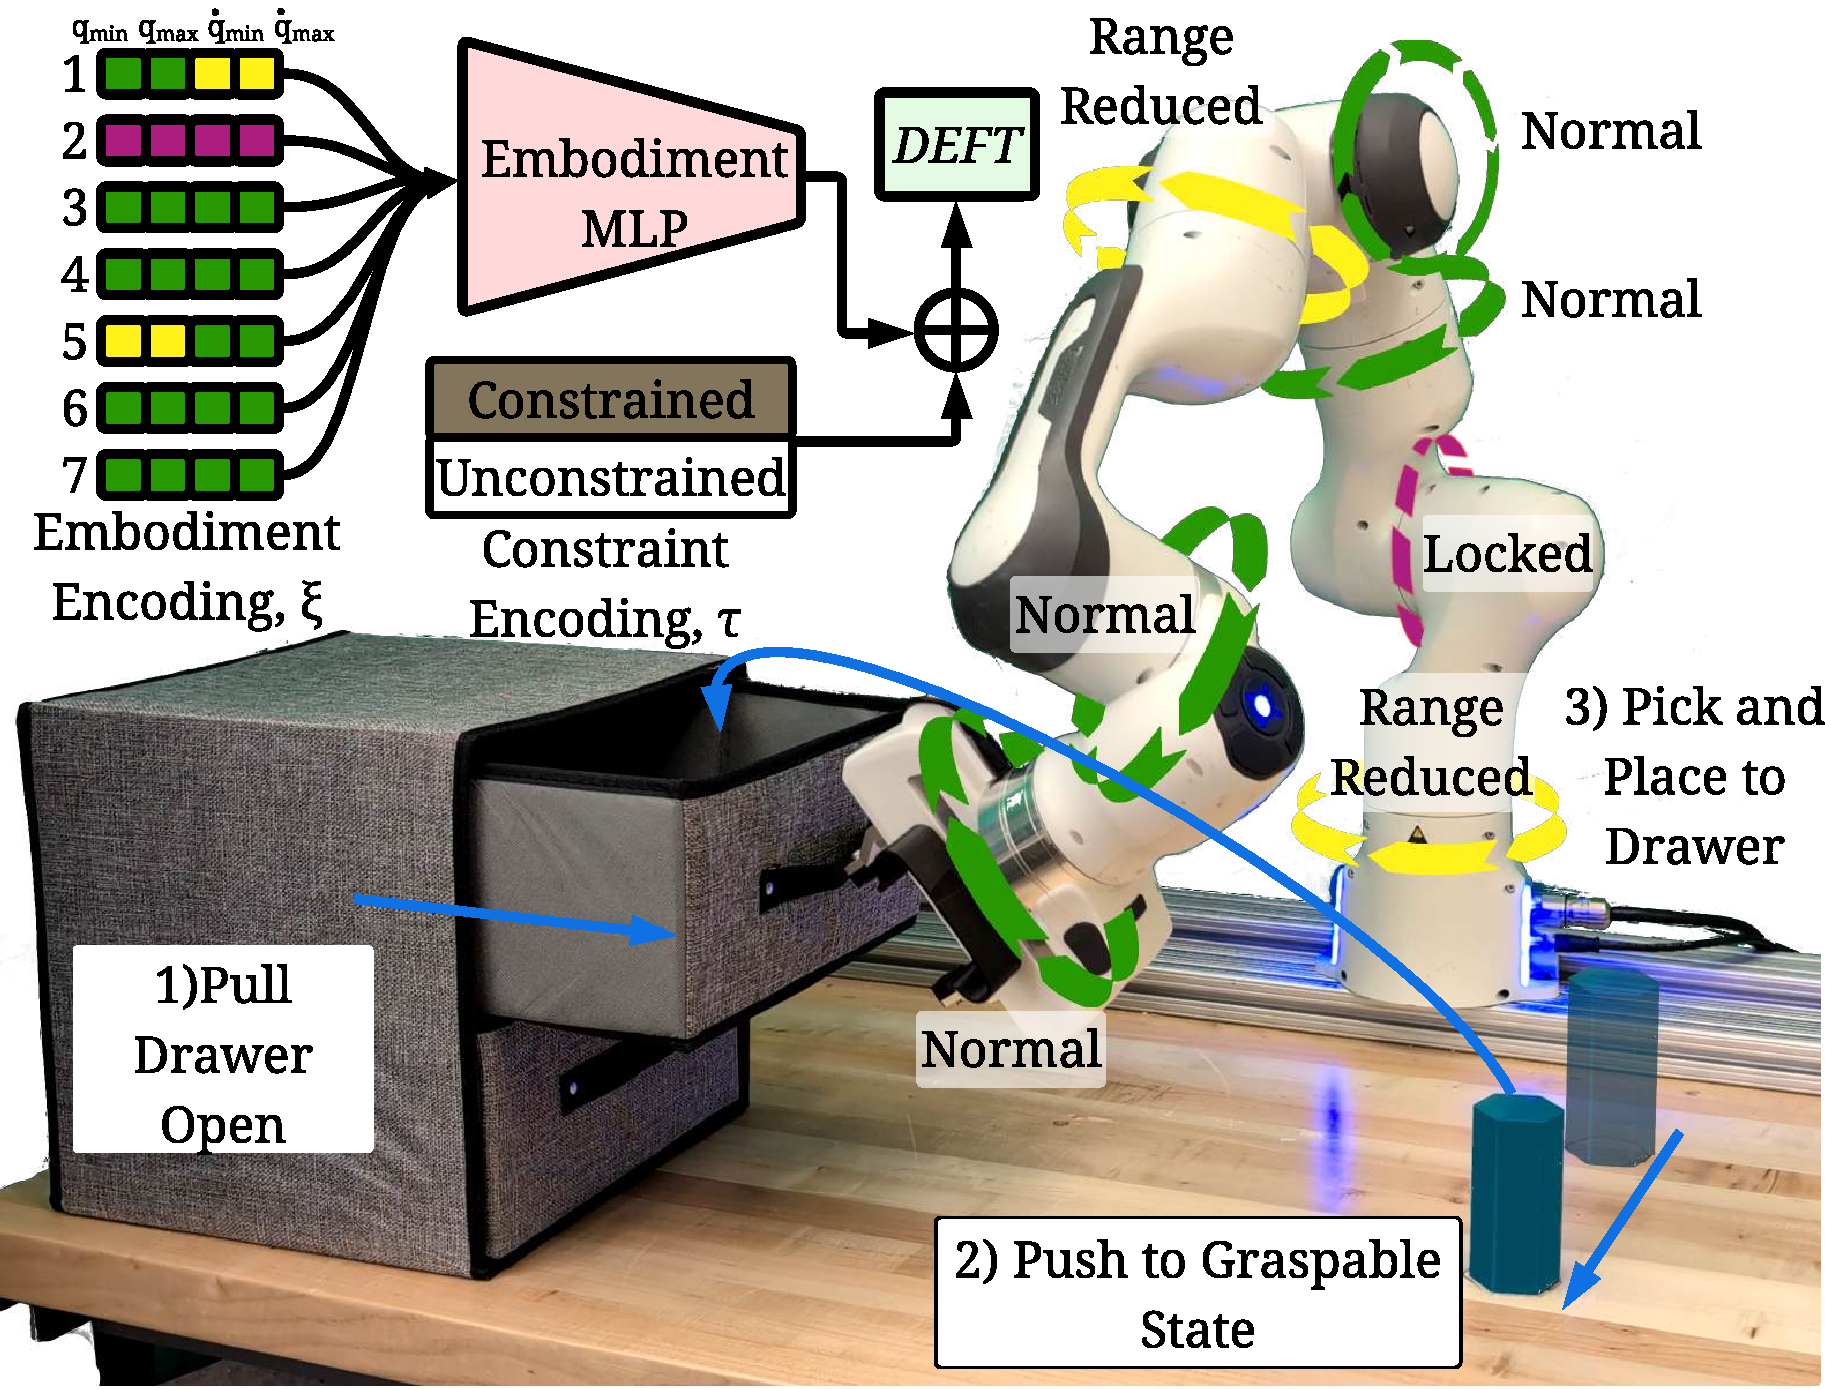
\includegraphics[width=\columnwidth]{figures/first_page_figure_compressed.pdf }
    \caption{DEFT takes as input a structured embodiment encoding representing joint-level failures and a constraint encoding then synthesizes a feasible robot trajectory via a diffusion model. After experiencing a failure, a given task will likely need to be completed in a different manner. In this figure, the pick-and-place segment is no longer feasible, given the failure condition of a locked second joint and reduced velocity range on joint 1 and reduced angle range on joint 5, and the robot must now push the object to a graspable state to complete the task. \vspace{-10pt}}
    \label{fig:first}
\end{figure}



In this work, we focus on \textit{actuation failures} as they directly affect how the robot moves. \textit{Fail-active} operation requires adapting to these altered kinematics, which can cause end-effector motion to become non-holonomic; meaning the same control input may no longer yield the same end–effector motion \cite{Bloch_Krishnaprasad_Murray_2016}. 
%
It is also important to note that since degradation can evolve over time \cite{barbieri2015sensor} and the failure state is not known a priori, \textbf{the space of failure modes is effectively unbounded}. Moreover, each joint can fail independently in multiple ways, and this complexity scales combinatorially with the robot’s degrees of freedom, \textbf{making reliable performance across failures hard to engineer}.

As failure-induced constraints redefine the robot's workspace, manipulability, and feasible interactions with the world, \textsl{we posit that each failure mode can be interpreted as a new embodiment}.  
% \ar{add a filler that describes why and what this means}
% We posit that failure could be interpreted as an embodiment shift: \ar{describe}
% Further, under embodiment shifts introduced by failure, 
% \ar{then, transition into multi-skill behaviors}
% \ar{under this lens, if you have differnet embodiments, not the same embodiment can perform that same tasks}, so
Through this lens, different embodiments are unable to perform the same tasks using the same behaviors. As no same set of behaviors can span all embodiments, multiple motion primitives are needed to expand the feasible action space and reachable task-space \cite{briscoe2024exploring}.
%so maintaining performance requires switching behaviors . 
For example, in \cref{fig:first}, reduced ranges on two joints and one locked joint prevents the robot from grasping the object. However, first pushing the object into a graspable pose and then picking-and-placing it inside the drawer, makes the task feasible.


% To this end, we must utilize motion primitives. Primitives provide compact, task aligned structure that encodes the right constraints for each family (e.g., free–space transfer vs. contact–guided alignment), and enables rapid switching when failures shrink workspace or alter feasible contacts. 

%Despite its importance, building fail-active robots is under-explored. 
Synthesizing effective motion primitives for arbitrary failure conditions is challenging due to the complex relationship between robot embodiment constraints and feasible task-space behaviors. Existing approaches fall short in three key gaps: 1) they do not generalize to arbitrary failure configurations \cite{briscoe2024exploring, xie2021maximizing}; 2) they are not capable of completing multiple manipulation primitives \cite{pham2024adaptive}; and 3) they do not address multi-joint failures \cite{mu2016kinematic, kim2024quadrupedal}. To the best of the authors’ knowledge, no existing work bridges all three of these gaps simultaneously. 
%\ar{why is it hard to address all 3 concerns simultaneously?}
Under the interpretation of failure as embodiment shift, these capabilities have not been realized as there are potentially infinite embodiments to generalize across and each embodiment has its own distribution of actions capable of achieving a set task. 
%The motion primtives combined with the infinite space of actuation failures results in a complex and multimodal trajectory distribution. 
% Diffusion models are well suited to such settings, capturing the distributions and retaining them when generating the trajectories.
Diffusion models are uniquely suited to solve this. Because they excel at modeling multimodal data distributions, diffusion policies can generate across the range of actions required to span these infinite embodiments at inference.

To this end, we present \textit{DEFT}: a \textit{D}iffusion-based \textit{E}mbodiment-aware \textit{F}ail-active \textit{T}ask-conditioned trajectory generation framework, capable of maintaining robot manipulation functionality under failure conditions. Our contributions are:
(i) an \textit{embodiment vector} encoding per-joint actuation failures for online adaptation to previously unseen failure-induced embodiments and
(ii) a \textit{constraint encoding} selecting between constrained and unconstrained motions to enable the use of multiple motion primitives.
%The conditioning on the primitive helps us push diffusion policy to the correct modes. 
Furthermore, we utilize start–goal inpainting and output clamping to enforce embodiment failure conditions \cite{repaint_lugmayr_2022}.
%the conditioned model achieves robust performance in real world scenarios. 
This allows \textsl{DEFT} to: 1) generalize to arbitrary failure configurations; 2) complete multiple manipulation primitives; and 3) handle multi-joint failures.
% We benchmark DEFT against conventional motion planning approaches, showing significant improvement in trajectory generation with arbitrary failures, obeying primitive constraints in the generated motion, and generalization to out-of-distribution failures.
We benchmark DEFT against conventional and learning based motion-planning approaches and demonstrate significant improvements in trajectory generation under arbitrary failures (up to 84\% success), adherence to task constraints (up to 78\% success), and generalization to previously unseen failures (up to 99\% success). Collectively, these results enable reliable fail-active operation, allowing robots to maintain functionality and safely complete tasks without human intervention across arbitrary failure conditions.

\vspace{-15pt}
% As deployments scale, even rare faults accumulate; \ar{<- I don't understand this} stopping for each event erodes uptime and undermines long-horizon autonomy. 
% This ability is necessary for the deployment of reliable robots, especially where intervention is costly or impossible.  
  % \ar{<- this seems a repetition of somethign you said already} 
% The number of unique robots only continues to grow exponentitially, and this growth is being buoyed by the introduction of robot motion planning polcies trained on multiple robots. Yet, one of the key challenges for their operation is the need to train or fine-tune for specific embodiments.
% Cross-embodiment policies tackle two modalities: human to robot and robot to robot. \gm{cite} However, we can define a third cross embodiment problem: failure-induced embodiment shift. Failures are inevitable over long deployments: wear, sensing drift, and partial actuation limits accumulate, altering the realized embodiment and invalidating nominal policies (\cref{applsci,mer90sols,msl_fmwi}). Human-in-the-loop recovery is slow, costly, and often impractical in remote or high-throughput settings, where downtime directly erodes mission and production value (\cref{applsci}). 
% Despite its importance, building fail-active robots is under-explored. In this work we focus on actuation failures as they are uniquely disruptive: they directly alter how the robot moves. Such joint-level failures, including reductions in angle or velocity range, cause complex and highly nonlinear changes to the mapping between control-space inputs and task-space outcomes \cite{Bloch_Krishnaprasad_Murray_2016}. Since, there exists an effectively infinite number of ways a robot can fail, and each unique failure condition may be interpreted as a new embodiment of the robot. 
% 
% % There are three key considerations of robot actuation failures: 1) degredation occurs continuously \cite{barbieri2015sensor}, 2) the failure state of the robot is not known a priori, and 3) there exists an effectively infinite number of ways a robot can fail, and each unique failure condition may be interpreted as a new embodiment of the robot. 
% 
% With the widespread development of cross-embodiment learning based approaches this natrually lends itself to the problem. But existing approaches take a train and fine-tune approach \cite{nvidia_gr00t_2025}, which requires additional expert demonstrations for the specific embodiment, or a model trained per embodiment \cite{chi2023diffusion}, or engineer in embodiment understanding \gm{cite body transformer}. These cannot address the three key considerations of actuation failure.
% Despite its importance, building fail-active robots is under-explored. We focus on actuation failures because they directly alter how the robot moves: joint-level range and velocity caps (or locks/torque limits) induce highly nonlinear changes in the mapping from control inputs to task-space outcomes \cite{Bloch_Krishnaprasad_Murray_2016}. 
% 
% \ar{again , you don't say why its' hard, you just say it's not explored} 
% \ar{need to impvover here. You want to plant the flag but you are not doing it well enough}

%conditioned explicitly on the selected motion primitive and the robot’s failure-induced embodiment constraints.

% \gm{we dance around it a lot and don't say it explicitly: We need to motivate diffusion because 'the complex relationship between
% robot embodiment constraints and feasible task-space behaviors', each mode can be viewed as a new embodiment of the robot (multimodal distributions, say this exactly), primitives also make it a multimodal distribution. }
% Conditioning on a small set of primitives reduces sample complexity, guides the denoiser toward the appropriate constraint manifold, and yields plans that remain feasible under failure–induced embodiment changes \cite{Huang2021}. 
% In practice, we use two primitives—\emph{transport} and \emph{guide}—as building blocks for varied manipulation tasks, and learn a single policy that selects and instantiates them under changing joint limits and velocities. 
% Prior work shows that enabling fail-active behavior may require robots to switch between alternative manipulation behaviors (e.g., from pick-and-place to poking or pushing), each inducing distinct classes of task-specific interactions .

% Treating each actuation fault as a morphology shift;  tightened joint limits, altered Jacobian conditioning, or partial torque loss; makes cross-embodiment methods a natural fit.

 % Viewing failure as a new embodiment suggests borrowing tools from cross-embodiment learning. However, common strategies have limitations for fault response: (i) train-then-fine-tune VLA create robot-specific policies when adapting to a new embodiment (post-training per platform) \cite{nvidia_gr00t_2025}, (ii) per-embodiment policies deliver high in-distribution reliability but offer little zero-shot transfer \cite{chi2023diffusion}, and (iii) engineered embodiment understanding (e.g., representation alignment) can improve transfer yet still presumes a stable morphology rather than a drifting failure state \cite{wiut24}.

% \ar{again, you don' say what  you do}
% \gm{explicitly what we do is diffusion for failure recovery and then add an additional conditionning vector to diffusion to close the sim to real gap: it's a vector of joint limits and a vector telling it whether to constrain the ee orientation and motion to a straight line or not. We need to re include primitive motivation (my prior work) and do a good job at saying why constrained motion is interesting to test}
% \gm{latest note: sim2real is hard, we got good results in sim using diffusion instead of optimization like existing approaches but gap in real world and conditioning helped close it, we did diffusion -> sim to real gap -> needed embodiment conditioning}
% Robots are becoming increasingly ubiquitous, being used in applications ranging from healthcare, to space, to high-mix warehouse automation. .facto}Current standards enforce \textsl{fail-freeze} behavior: robots must halt operation when faults are detected \cite{ISO10218-1, ISO13849-1, IEC60204-1}. 
% On Mars, months-long and even multi-year recoveries are routine. Opportunity’s robotic arm shoulder motor first stalled on November 25, 2005, prompting workarounds and continued management of intermittent stalls years later; Curiosity’s drill feed fault halted coring from December 2016 until May 2018, when a new feed extended drilling method restored sampling. These episodes illustrate that faults in continuously operating systems are inevitable \cite{factory_efficiency_2020}. Current standards enforce \textsl{fail-freeze} behavior: robots must halt operation when faults are detected \cite{ISO10218-1, ISO13849-1, IEC60204-1}. In this work, we borrow the term \textsl{fail-active} from the aerospace community as a long-term goal for robots, defined as the ability to function completely or in a reduced manner in the event of a failure \cite{aero_reliability}.  


%Robots are on the cusp of ubiquity in the real world, enabled by their growing physical ability and the success of end-to-end models that allow them to perform many tasks effectively \gm{put some good cites}. However, one major impediment to mass adoption is the inevitability of hardware failure. When a hardware fault is detected, current standards recommend that robots \textsl{fail-freeze}: stop operation when a fault is detected. \cite{ISO10218-1, ISO13849-1, IEC60204-1}  This stands in stark contrast to other mechanical systems, such as automobiles and aircraft, that are \textsl{fail-active}: able to continue to perform its function with a failure occuring. \cite{aero_reliability} The need to halt operations in robots experiencing a fault is fundamentally incompatible with use cases where continuous operation despite hardware faults is essential such as: surgical robots, space and remote robots, and future utilitarian robots.

%There are many components in a robot that can fail \gm{cite one of the old long-term study papers}, but in this work we focus on failures that affect the actuation of the joints. Failures in the joints are of particular importance because they warp the coupling of the configuration and task spaces in non-linear ways. \cite{Bloch_Krishnaprasad_Murray_2016, atreya_steering}. Joint failures can manifest in a number of ways: such as through actuator failures that limit joint velocity, acceleration, or range, or result in joint locking. Compensating for the failures is made more difficult by the near-infinite space of possible failure configurations: each joint may independently experience varying limits on position, velocity, or acceleration, and the robot must adapt through compensatory behaviors that grow combinatorially with the number of degrees of freedom. Handling such failures requires motion planning systems that solve a dual problem: 1) understanding how failure constrains trajectory generation, and 2) being aware of the requirements of the task that the robot is to complete to serve its function.

%Prior work in has shown that being fail-active to joint failures in task space necessitates the use of an expanded set of manipulation behaviors in order to complete the tasks commanded of the robot. \cite{briscoe2024exploring}. This paper will adopt this paradigm to enable fail-active task planning. Pick and place can become infeasible under certain failures, but other approaches, such as poking and pushing, can still work. 

%Each of the two prior problems consist of trajectories that belong to a unique distribution. and going across distributions is hard. Each modality of motion primitive has a unique joint trajectory distribution that forces it to be the class of motion in the end effector. Each failure changes the limits in some way that non-linearly maps to changes in the task space, so each failure for each joint for each type represents its own distribution of trajectories. Defining these constraints empirically is exceedingly difficult and infeasible, but we can learn to condition some information of the failure and of the task in order to produce trajectories in and across these distributions. Diffusion is good at this because it can learn a conditional model of trajectories given some information about the trajectory. 

%Using all this, the contributions of this work are:
%\begin{itemize}
 %   \item A definition of a more general set of failures, including full, partial, reduced velocity, and reduced acceleration, to address than any prior work
    %\item A meaure of the affect of failures have on the robot's task capability
    %\item The ability to generate failure constrainted trajectories
    %\item The ability to create task-specified actions with failures
%\end{itemize}


% To deploy robots in unstructured or remote environments over long time horizons—on the order of years—we must develop systems that can automate this graceful degradation. We define this capability as fail-active: the ability for a robot to continue operating even as its embodiment degrades, such as through actuator failures that limit joint velocity, acceleration, or range, or result in joint locking. Handling such failures requires motion planning systems that incorporate embodiment-specific constraints directly into trajectory generation.

% This challenge is made more difficult by the near-infinite space of possible failure configurations: each joint may independently experience varying limits on position, velocity, or acceleration, and the robot must adapt through compensatory behaviors that grow combinatorially with the number of degrees of freedom \gm{cite or rephrase if needed}. Despite the inherent flexibility of diffusion-based planning approaches, most prior work assumes a constant embodiment. In contrast, we embed embodiment-conditioned adaptability into a diffusion model, enabling it to generalize over multimodal distributions of joint capabilities and failure states.

% Because the relationship between control actions and joint motion becomes increasingly nonlinear under embodiment changes, diffusion models are well-suited to this problem. Just as they are able to model multiple valid solutions for complex real-world tasks, they are also capable of capturing diverse strategies for achieving a task across various physical degradations. Our approach extends this flexibility, offering a step toward scalable and resilient robot autonomy.

% For robots to remain effective over long time horizons---on the order of years---they must adapt to inevitable physical degradation. In high-stakes contexts such as space or remote exploration, maintaining operational capability is critical, as physical repairs and human intervention are infeasible\gm{cite}. 



% In this paper, we enable robots to be fail-active, defined as the ability to continue operation when the physical form of the robot degrades, in the face of actuator failures. Actuator failures, including decreased joint velocity and acceleration, reduced angle range, or full locking, requires trajectory generation approaches that incorporate these changes in the embodiment while planning for tasks \gm{cite if possible}. This difficulty is compounded by the near-infinite space of possible failure configurations, where each joint may experience varying constraints on position, velocity, and acceleration, and the compensatory degrees of freedom grow combinatorially with the complexity of the robot \gm{rewrite this sentence}. State-of-the-art failure recovery methods only address single joint failures and limited types of failures\gm{cite}. To truly enable a robot to be fail-active, the robot's motion planning system must be able to adapt to any change in the robots abilities. Without addressing this challenge, long-term autonomy in unstructured and remote environments may remain out of reach. 


% Existing work in fault-tolerant motion generation fall into three categories: 1) pre-computation, 2) analytical inverse-kinematics, and 3) learning-based methods. Pre-compuation creates a limited set of task-specific motions, which restricts their ability to adapt to new or unforeseen failure configurations \citep{briscoe2024exploring}. Approaches based on analytical inverse kinematics require hand-crafted, embodiment-specific models and are limited to single failure modes at a time \citep{mu2016kinematic, lewis1997fault}. Learning-based methods, such as reinforcement learning, have demonstrated the ability to compensate for joint impairments but are typically restricted to specific robot morphologies or failure types \citep{pham2024adaptive, kim2024quadrupedal}.  When the robot's embodiment degrades, this task and action separation creates a mismatch between planned and executed motions \gm{cite}.

% Existing methods are inadequate because they are not truly generalizable to arbitrary failures. They are unable to handle combinations or multiple types of actuator failures. The core challenge is to develop a trajectory generation model that can compensate for arbitrary failures while remaining capable of generating feasible trajectories under real-world environmental constraints. An ideal solution would take in the failure state of the robot, alongside task and environmental information, and generate valid, executable trajectories without needing retraining or post-processing. 
% Diffusion models — with their ability to model multimodal distributions and generalize across varying conditions — are particularly well-suited to address this challenge. For instance, industrial arms like the KUKA LBR iiwa are rated for approximately 30,000 hours of operation, or about 3.5 years \citep{kuka_lbr_iiwa}.

% In this paper, we introduce a diffusion-based trajectory generation framework that is explicitly conditioned on the robot's embodiment data. Diffusion models are well-suited to this problem because they can model complex, multimodal distributions — in this case, the space of feasible robot trajectories under varying kinematic constraints. The key insight is that by conditioning the diffusion model on the robot’s joint limits (position, velocity, and acceleration), the model can generate multiple feasible solutions even under unseen failure scenarios. Unlike traditional methods that require that are tailored to specific failure modes, our approach allows the model to adapt to new actuator constraints at inference time despite being trained on a finite set of failures. We adopt a diffusion policy framework \citep{chi2023diffusion} and extend it to handle embodiment conditioning by integrating two key mechanisms: (1) direct conditioning of joint angle, velocity, and acceleration limits, and (2) clamping the denoised trajectory at each diffusion step to ensure that the generated joint states remain within the specified limits. This approach enables generalization to unseen embodiments and failure modes at inference time without requiring failure-specific or task-specific retraining or separate post-processing to enforce feasibility. To the best of our knowledge, this is the first approach to successfully condition a diffusion model on actuator data to handle both kinematic and dynamic failures concurrently — including complex scenarios where joint angle and velocity limits are restricted simultaneously. We evaluate our approach over a set of basic motion primitives, demonstrating robustness over increasingly disabling failures. We further performed an ablation study to demonstrate the need for each part of the conditioing and clamping of the diffusion model \gm{do better}.



% We are on the cusp of having robots operate in the real world en masse (cite hyundai buying 10k humanoids) because they are able to do many tasks well using an end-to-end models because they are so physically complex
% An impediment to universal adoption is the enevitable failure of the hardware of the system 
% right now iso recommends stopping system when a fault occurs --- that is not scalable
% that is in stark contrast to humans that are able to compensate to complete tasks when injured
% An existing example is the mars rover arm failing quickly after 
% we want to make systems that are able to adapt and continue operating when they have degradation (graceful degradation)
% existing diffusion approaches (and motion planning at large) expect a constant embodiment, despite their inherent flexibility, we put that flexability in
% because the relationship between actions and joint motions changes non-linearly with changes in joint capability, we need to use diffusion because it can have the multimodal distribution understanding

% for the same reason they are able to handle multiple complex tasks in the real world, they are able to handle multiple system failure states to complete the same task
\section{Related Work}% \gm{We have the space to add narrative commentary in here}% 
% train model per embodiment:
% \cite{co24, ACT23, to24, xo24}
% Train and fine-tune per embodiment:
% \cite{pi_0_24, chen_conrft_2025, wzltsf25-1, kim_openvla_2024, yo24, shukor_smolvla_2025, wzltsf25, nvidia_gr00t_2025, wiut24, yo25}

% Policies Engineered for Cross-Embodiment: \cite{bogert_built_2024, yzfl24, freiberg_diffusion_2024, chen_graphmimic_nodate, lo24-1, yo25}

% Latent Space Policies:
% \cite{wo25-1, bauer_latent_2025}

% Others:
% \cite{seo_masked_2023, yang_pushing_2024, ldb25}

% Cross-embodiment learning seeks to develop control policies that function across heterogeneous robot bodies—i.e., differing morphologies, kinematics, sensors, and actuators—so that capability does not have to be relearned from scratch for each platform. train model per embodiment specialized, robot/task-specific policies that optimize in-domain performance without explicit transfer guarantees \cite{co24, ACT23, to24, xo24}. \emph{Train and fine-tune per embodiment}—generalist VLAs/flow models pretrained on diverse multi-robot data and adapted to each target via PEFT or brief online updates, balancing reuse with hardware specificity \cite{pi_0_24, chen_conrft_2025, wzltsf25-1, kim_openvla_2024, yo24, shukor_smolvla_2025, wzltsf25, nvidia_gr00t_2025, wiut24, yo25}. \emph{Policies Engineered for Cross-Embodiment}—representation alignment, shared interfaces, and cross-domain co-training that aim for one policy spanning morphologies \cite{bogert_built_2024, yzfl24, freiberg_diffusion_2024, chen_graphmimic_nodate, lo24-1, yo25}. \emph{Latent Space Policies}—robot-agnostic action/interaction spaces that unify end-effectors and enable transfer with thin adapters \cite{wo25-1, bauer_latent_2025}. \emph{Others}—complementary lines on masking, scaling across embodiments, and broad evaluation \cite{seo_masked_2023, yang_pushing_2024, ldb25}.
% Cross-embodiment in robotics addresses the fact that skills learned on one robot rarely transfer to another because morphologies, sensors, and action spaces differ; the aim is to reduce per-robot data/compute and enable policy reuse across hardware. At one end, some works train a model per embodiment—specialized robot- and task-specific policies that maximize in-domain reliability, with occasional use of intermediate interfaces like object flow to bridge human/sim data to a target platform \cite{co24, ACT23, to24, xo24}. Another line pretrains generalist VLA or flow models on heterogeneous multi-robot corpora and then fine-tunes them for each target with parameter-efficient updates or brief online RL, yielding dependable last-mile adaptation while retaining broad priors \cite{pi_0_24, chen_conrft_2025, wzltsf25-1, kim_openvla_2024, yo24, shukor_smolvla_2025, wzltsf25, nvidia_gr00t_2025, wiut24, yo25}. A complementary direction deliberately engineers morphology-robust interfaces and representations—tactile shared interfaces, gripper-agnostic encoders with geometry-aware decoders, graph abstractions, adversarial decomposition, and unsupervised cross-embodiment pretraining—so a single policy or pretrained backbone can span mismatched bodies with only thin adapters \cite{bogert_built_2024, yzfl24, freiberg_diffusion_2024, chen_graphmimic_nodate, lo24-1, yo25}. Finally, latent-space policies learn a robot-agnostic interaction/action latent and pair it with lightweight embodiment decoders or hand descriptors, enabling one controller to serve multiple end-effectors with minimal retraining \cite{wo25-1, bauer_latent_2025}.
% Cross embodiment addresses the gap where a skill trained on one robot embodiment often fails on another. This is because embodiment, sensing, and action spaces 
% differ. A well established line of research is to train a model per embodiment, prioritizing reliable in domain performance and, when leveraging external data,  and occasionally using intermediate interfaces  to bridge datasets and  \cite{co24, ACT23, to24, xo24}. Other works pretrain generalist VLA or flow matching models on heterogeneous multi robot dataset \cite{pi_0_24, chen_conrft_2025, wzltsf25-1, kim_openvla_2024, yo24, shukor_smolvla_2025, wzltsf25, nvidia_gr00t_2025, wiut24, yo25}. They then fine tune each model for the target robot with parameter efficient updates or brief online RL, reusing broad priors while delivering dependable last mile performance. Another direction engineers embodiment robust interfaces and representations. Examples include tactile shared interfaces, gripper agnostic encoders with geometry aware decoders, graph based video abstractions, adversarial decomposition, and unsupervised cross embodiment pretraining, enabling one policy or a pretrained backbone to span mismatched robots with only thin adapters \cite{bogert_built_2024, yzfl24, freiberg_diffusion_2024, chen_graphmimic_nodate, lo24-1, yo25}. Finally, latent space policies learn a robot-agnostic interaction or action latent and pair it with lightweight embodiment decoders or hand descriptors, enabling one controller to serve multiple end effectors with minimal retraining \cite{wo25-1, bauer_latent_2025}.





% \gm{add papers I want to cite}
% \subsection{Embodiment Failure Recovery}

% Robots operating over long horizons in uncertain environments must cope with degradation to their physical embodiment, including joint locking, reduced range, and dynamic instability. Analytical approaches have addressed this by explicitly modifying motion planning and control algorithms to maintain function under such impairments. Techniques such as self-motion manifold intersection planning~\cite{xie2021maximizing}, fail-safe reachability analysis~\cite{porges2021failsafe}, and redundancy reconfiguration via closed-loop inverse kinematics~\cite{rayankula2021fault} aim to guarantee task success despite failures. Others use optimization-based control to exclude failed joints~\cite{yang2024qp}, derive inverse kinematics for specific locked-joint cases~\cite{wang2021ik}, or adapt control laws for stability under chaotic degradation~\cite{khan2023chaos}. These methods provide robust, explainable guarantees, but are often limited to single failure modes, require significant manual modeling effort, and do not scale easily to unseen configurations. \gm{fix this sentence, maybe make it two sentences, maybe incoproate/sprinkle the limitations throughout?}

% Design-time strategies aim to increase fault tolerance by optimizing kinematic structure itself~\cite{almarkhi2020design}, while task-specific gait reconfiguration for legged systems~\cite{xi2025gait} allows continued locomotion with partial joint paralysis \gm{note how a lot of these are on walking and some on point to point, but none on task solutions}. Collectively, these works show that it is possible to analytically adapt to embodiment failures when the robot model is known and the failure mode is anticipated. Our proposed approach takes a contrasting view: instead of hand-crafting failure-specific solutions, we use a data-driven generative model trained on diverse failure data to synthesize feasible, compensatory trajectories at inference time, potentially generalizing across multiple failure types and robots.

% \subsection{Learning-Based Failure Recovery}

% A growing body of learning-based work aims to overcome the limitations of handcrafted methods by training robust, generalizable policies. Reinforcement learning has been used to adapt to joint-level failures via adversarial training~\cite{yang2021adversarial}, partial observability~\cite{pham2024adaptive}, and random joint masking during locomotion~\cite{kim2024quadrupedal}. These strategies have proven capable of recovering from severe physical impairments, particularly in quadrupeds and manipulators. Policy architectures such as FT-Net~\cite{luo2023ftnet} and fault-conditioned networks enable recovery behaviors to activate automatically during failure. \gm{todo: weaknesses}

% Other strategies leverage curriculum learning to gradually expose the robot to increasing impairment severity~\cite{okamoto2022acdr}, or build behavior repertoires via quality-diversity search that can rapidly switch to a viable alternative after damage~\cite{cully2015qd, allard2023hierarchical} \gm{double check the exact method cully uses}. While these approaches often demonstrate strong performance, they typically rely on task-specific training pipelines and either explicit retraining or policy selection at runtime. In contrast, our diffusion-based model learns a generative distribution of full trajectories over failure modes, allowing flexible inference-time adaptation without online optimization or policy switching.
\paragraph{Failure-Aware Robot Control}

Robots operating over long durations in uncertain environments must be able to continue functioning even when experiencing physical degradation. Joint-level failures, such as locking, reduced range of motion, or diminished velocity, introduce complex, nonlinear constraints that disrupt standard motion planning approach. Classical methods attempt to address these challenges through explicit algorithmic adaptation: self-motion manifold planning~\cite{xie2021maximizing}, fail-safe reachability analysis~\cite{porges2021failsafe}, and redundancy exploitation via inverse kinematics~\cite{rayankula2021fault}. In assuming a subset of possible failures, these approaches offer guarantees on post-failure ability but they are unable to extend to arbitrary failure conditions. Other works adapt control laws to handle specific joint failures~\cite{yang2024qp, wang2021ik, khan2023chaos}, but are often limited in generality, scale poorly with the combinatorial space of failure types, and rely heavily on manual modeling. While effective in narrow domains, these handcrafted solutions cannot address the full complexity of real-world fail-active behavior, where failures must be handled, and task strategies adapted, on the fly.

% Learning-based strategies aim to overcome the limitations of traditional methods by training control policies that adapt to embodiment changes through experience. In reinforcement learning, damage-aware behaviors have been demonstrated via adversarial training~\cite{yang2021adversarial}, partial observability~\cite{pham2024adaptive}, and stochastic joint masking~\cite{kim2024quadrupedal}. Other approaches use curriculum learning~\cite{okamoto2022acdr} or quality-diversity search~\cite{cully2015qd, allard2023hierarchical} to build behavioral repertoires capable of failure recovery. 

Learning-based strategies address the limitations of traditional methods by training control policies that adapt to embodiment changes through experience. In reinforcement learning, damage-aware behaviors have been achieved using adversarial training \cite{yang2021adversarial}, partial observability \cite{pham2024adaptive}, and stochastic joint masking \cite{kim2024quadrupedal}. Other methods apply curriculum learning \cite{okamoto2022acdr} or quality diversity search \cite{cully2015qd, allard2023hierarchical} to develop behavioral repertoires for failure recovery.
These techniques have shown success in recovering locomotion or point-to-point reaching under known embodiments, but often require task-specific training loops, explicit policy switching, or runtime optimization. 
% More importantly, no existing method generalizes across multiple manipulation primitives or failure configurations without retraining. 
In contrast, our approach trains a generative diffusion model over full trajectories, enabling flexible, zero-shot adaptation to joint degradation and task shifts without policy switching or fine-tuning.

\paragraph{Diffusion Models for Trajectory Generation}
Diffusion models offer key advantages for trajectory generation in fail-active robotic systems, especially when embodiment changes unpredictably. Compared to imitation or reinforcement learning, diffusion models (1) capture complex, multimodal action distributions essential for recovery behaviors \cite{chi2023diffusion}, (2) provide stable training, outperforming alternatives like energy-based models \cite{zhong2023edmp}, and (3) enable conditional generation on structured inputs such as goals or embodiment states \cite{yang2023dimsam}. These features allow robots to adapt to joint failures without explicit retraining.

Empirically, diffusion models excel in robotic tasks like navigation, manipulation, and object rearrangement \cite{sridhar_nomad_2023}, outperforming reinforcement learning and behavior cloning in long-horizon, contact-rich tasks \cite{dasari_ingredients_2024}. Advances in diffusion transformers, like adaptive normalization and efficient tokenization, further enhance their suitability for continuous control \cite{dasari_ingredients_2024}. Crucially, diffusion supports online adaptation via trajectory reconditioning, enabling flexible fail-active responses without policy switching \cite{zhong2023edmp}, making them ideal for handling joint failures that reshape the motion space.


% Diffusion models offer key advantages for trajectory generation in fail-active robotic systems, particularly where the robot's embodiment can change unpredictably. Compared to conventional imitation or reinforcement learning methods, diffusion models (1) capture complex, multimodal action distributions essential for diverse recovery behaviors \cite{chi2023diffusion}, (2) maintain stable and reliable training dynamics,even relative to alternative generative methods like energy-based models \cite{zhong2023edmp}, and (3) enable conditional generation on structured inputs such as goals or embodiment states \cite{yang2023dimsam}. These properties are critical when robots must flexibly adapt to new constraints imposed by joint failures without explicit retraining or reprogramming.

% Beyond their architectural strengths, diffusion models have demonstrated strong empirical performance in real-world robotic domains including navigation, object rearrangement, and manipulation \cite{sridhar_nomad_2023}. Notably, they outperform reinforcement learning and behavior cloning in long-horizon, contact-rich tasks, where precise, multimodal reasoning is required \cite{dasari_ingredients_2024}. Recent advances in diffusion transformer architectures, such as adaptive normalization and efficient tokenization, further improve their viability for continuous control \cite{dasari_ingredients_2024}. Critically for failure recovery, diffusion models naturally support sampling-based online adaptation: they can recondition trajectories dynamically as embodiment constraints evolve, enabling flexible fail-active behavior without policy switching \cite{zhong2023edmp}. This makes diffusion particularly well-suited for real-world scenarios where joint-level failures redefine the feasible motion space and require rapid synthesis of new, task-complete trajectories.

\section{Methods}
\begin{figure*}
  \centering
  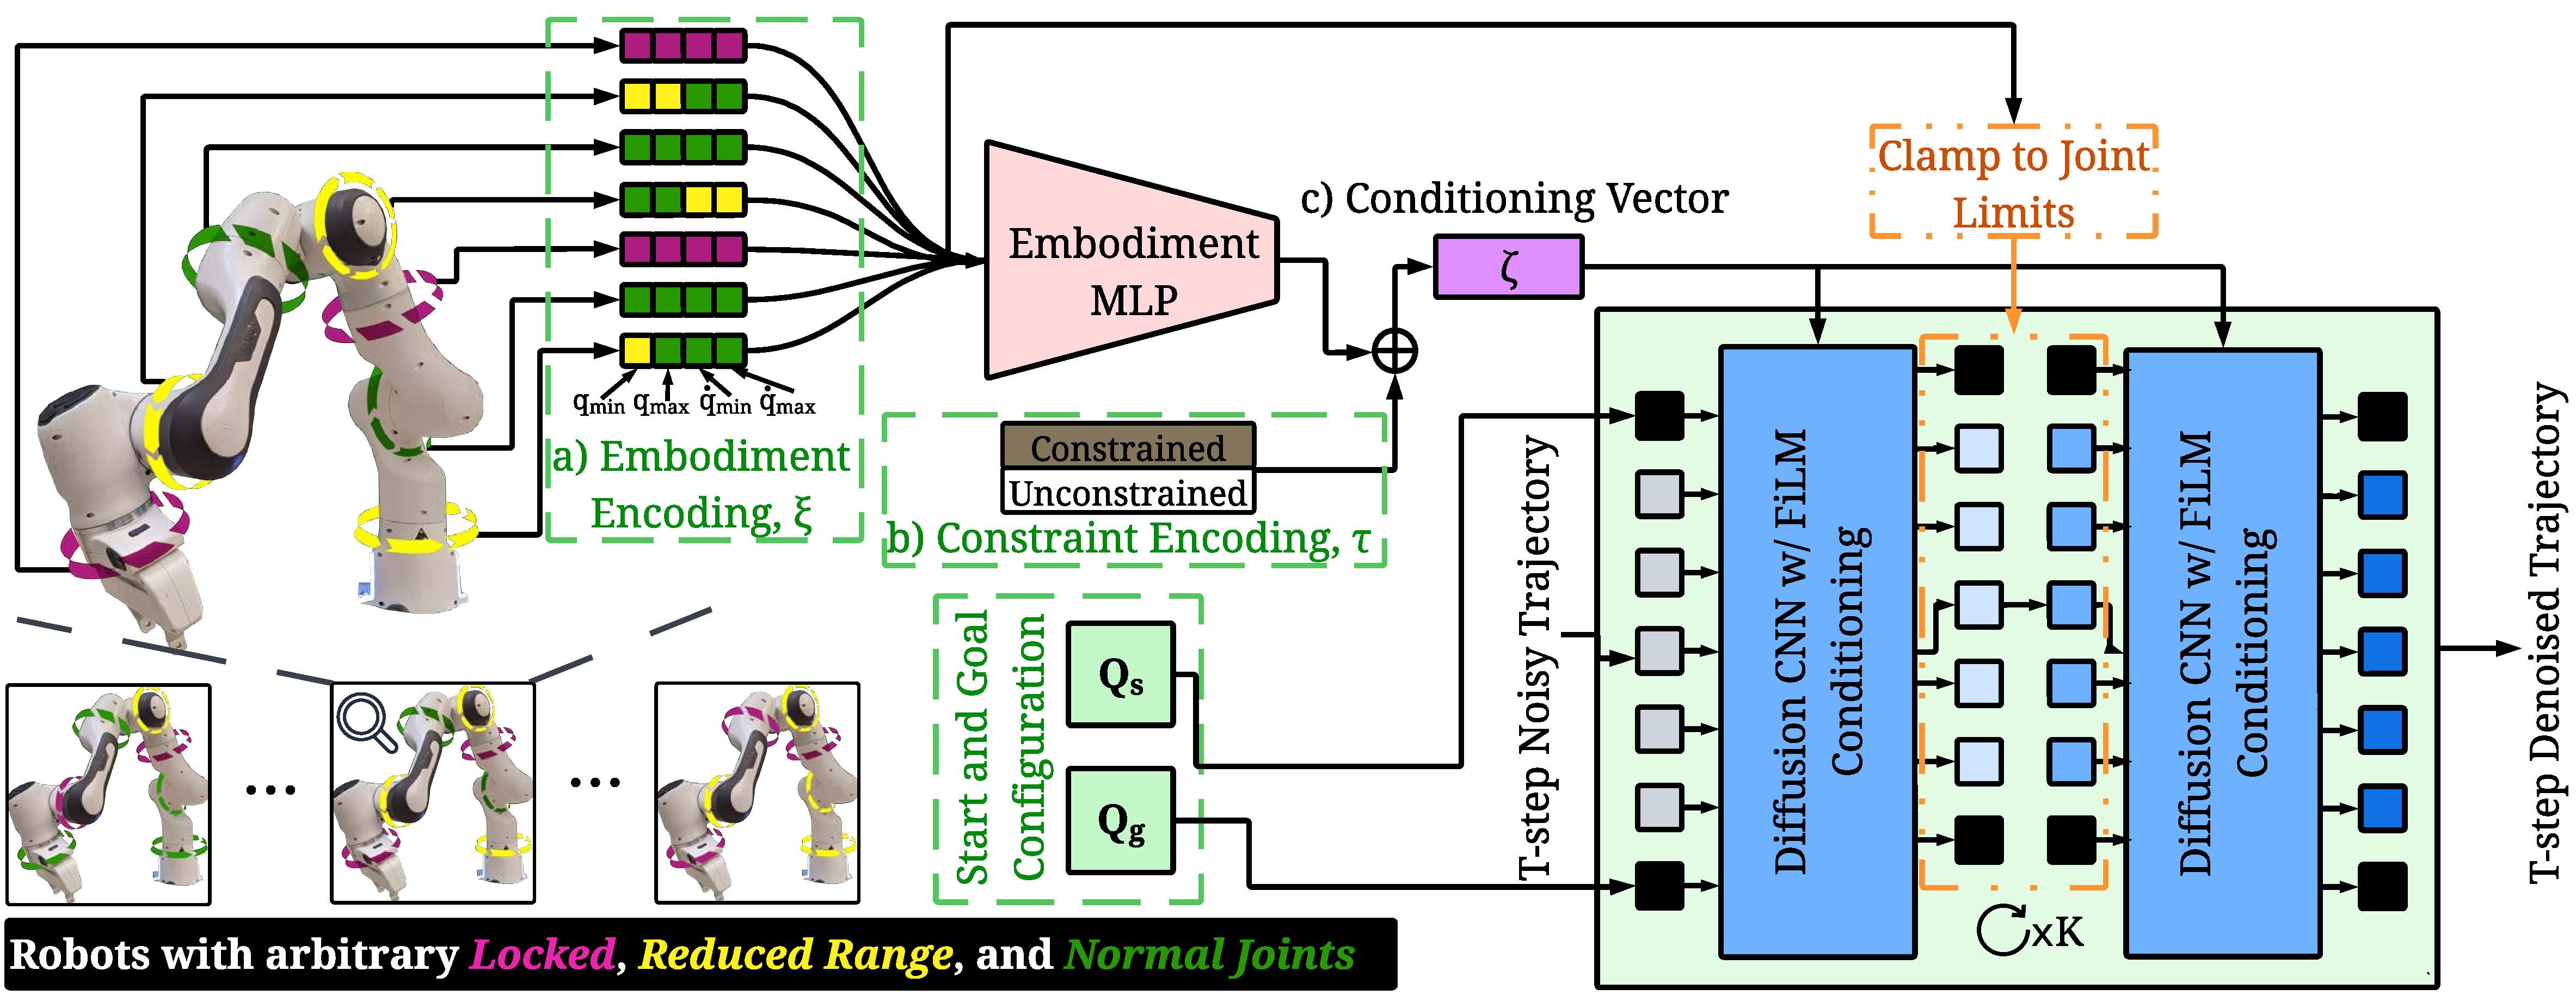
\includegraphics[width=\textwidth]{figures/block_diagram.pdf}
  \caption{Overview of DEFT. a) joint-level embodiment constraints are encoded into a structured representation capturing failure constrained joint position and velocity limits. This embodiment encoding is processed by a multilayer perceptron (MLP) and used to condition the diffusion model. b) Task-specific constraints (e.g. unconstrained or constrained) are represented as one-hot vectors and concatenated with the embodiment encoding to constrained the generative process. 
  Given these conditioning signals and start-goal joint configurations, the model generates feasible joint-space trajectories adapted explicitly to both the robot's degraded embodiment and task requirements. At each step of the denoising process the predicted joint values are clamped to the failure-induced robot joint limits. \vspace{-12pt}}
  \label{fig:system-diagram}
\end{figure*}
% \gm{Basically for the methods we need to describe only our contribution: diffusion for failure recovery, conditioning on embodiment, and conditioning on primitive, and inpainting (hardcoding but don't say this) the joint limits. We need to make sure this supports the narrative of 'diffusion rocks at failure recovery and we needed to add conditioning to close the sim to real gap'}

% \gm{We need: 1) an algorithm block on the diffusion approach, 2) plain english descriptions of \textbf{all} math, 3) remove unconstrained and constrained definitions}

% \gm{Finally, we need to write this methods section with reproducibility in mind. For another experienced PhD student, if they take this methods section, can they create our approach from scratch?}


% Our aim is to make robots fail-active by generating functional and feasible trajectories even in the event of joint-level failures.

% We frame this as a trajectory generation problem conditional on failure embodiment and task constraint. Each unique failure defines a new embodiment of the robot, and each task constraint (e.g., \texttt{unconstrained} or \texttt{constrained}) induces a distinct trajectory distribution. 
Our goal is fail-active manipulation: generate functional, feasible trajectories under joint-level failures. We pose this as conditional trajectory generation given the failure-induced embodiment and the task constraint. Each failure specifies a new embodiment of the robot, and each constraint (e.g., \texttt{unconstrained} vs. \texttt{constrained} motion) induces a distinct trajectory distribution. Given the start and goal joint configurations  the policy $\pi$ infers a future sequence of joint states over a fixed number of steps $T$. Unlike prior work that assumes a fixed set of failure configurations to control over, our method adapts online. It learns both the control behavior and the allowable motions from the current failure condition and the task constraint.
Our formulation enables zero shot trajectory generation across diverse embodiments and task conditions. For example, when a shoulder joint becomes unusable, the robot can switch from lifting to pushing an object without task specific retraining or policy switching.

\subsection{DEFT}
Inspired by recent advances in diffusion policies~\cite{chi2023diffusion}, we develop DEFT for an $N$-degrees of freedom robot to synthesize joint-space trajectories. Formally, the policy is defined as:
\begin{equation}
\pi(Q_{s,g}| \xi, \tau) \rightarrow \{\textbf{q}_{1:T}, \dot{\textbf{q}}_{1:T}\}
\end{equation}

The policy is conditioned on a vector $\xi \in \mathbb{R}^{4N}$ that encodes joint-level embodiment constraints imposed by the failure condition, and on a task constraint represented by a one-hot encoded vector $\tau$, as shown in \cref{fig:system-diagram}.

Given a ground-truth trajectory $\mathbf{x}$ and a diffusion time step, we first add Gaussian noise $\mathcal{N}(\mathbf{0}, \mathbf{I})$ to obtain a corrupted trajectory. We then inpaint the start and goal joint positions, $Q_{s,g} = [{(\textbf{q}_s, \dot{\textbf{q}}_s), (\textbf{q}_g, \dot{\textbf{q}}_g)}], q \in \mathbb{R}^N$, so endpoints remain exact. We proceed by clamping the entire noisy trajectory to the joint angle and velocity limits specified by the failure embedding $\xi = [\mathbf{e}_q, \mathbf{e}_{\dot{q}}] \in \mathbb{R}^{4N}$, ensuring feasibility under the current embodiment. Next, we form a conditioning vector, $\zeta = [\xi, \tau]^\top $,  by encoding the failure embedding with a small MLP and concatenating the resulting features to the task constraint token. The denoiser (UNet) receives the clamped, inpainted trajectory together with the time step and conditioning vector, and predicts a denoised trajectory $\hat{\mathbf{x}}$, denoising for $K=25$ steps as it showed no change in trajectory quality while having a inference speed improvement compared to \cite{chi2023diffusion}. Finally, we hard-enforce constraint adherence by clamping the prediction to the same limits and re-inpaint the endpoints, returning the denoised, feasible trajectory.


\subsection{Conditioning Approaches}
% \begin{algorithm}[t]
% \caption{Constraint-Aware Diffusion Step}
% \label{alg:diffusion}
% \KwIn{Ground-truth trajectory $\mathbf{x}$, timestep $t$, failure embedding $\mathbf{f}$, primitive encoding $\mathbf{p}$}
% \KwOut{Denoised trajectory $\hat{\mathbf{x}}$}
% Sample noise $\boldsymbol{\epsilon} \sim \mathcal{N}(0, I)$\;
% Compute noisy input: $\tilde{\mathbf{x}}_t = \sqrt{\alpha_t} \cdot \mathbf{x} + \sqrt{1 - \alpha_t} \cdot \boldsymbol{\epsilon}$\;
% \textbf{Inpaint} start and goal: $\tilde{\mathbf{x}}_t[\text{start/goal}] \leftarrow \mathbf{x}[\text{start/goal}]$\;
% \textbf{Clamp} $\tilde{\mathbf{x}}_t$ to limits specified by $\mathbf{f}$\;
% Fuse failure and primitive encodings: $\mathbf{c} \leftarrow \text{MLP}_f(\mathbf{f}) \, \| \, \text{MLP}_p(\mathbf{p})$\;
% Predict denoised trajectory: $\hat{\mathbf{x}} = \text{Unet}(\tilde{\mathbf{x}}_t, t, \mathbf{c})$\;
% \textbf{Clamp} output $\hat{\mathbf{x}}$ to limits in $\mathbf{f}$\;
% \textbf{Inpaint} start and goal: $\hat{\mathbf{x}}[\text{start/goal}] \leftarrow \mathbf{x}[\text{start/goal}]$\;
% \Return{$\hat{\mathbf{x}}$}
% \end{algorithm}
% Uses your existing \usepackage{algorithm} and \usepackage{algorithmic}
% \begin{algorithm}[t]
% \caption{\textit{DEFT}}
% \label{alg:diffusion}
% \begin{algorithmic}[1]
% \REQUIRE Denoising Steps $K$; Failure embedding $\mathbf{\xi}$; Primitive encoding $\mathbf{\tau}$
% \ENSURE Denoised trajectory $\hat{\mathbf{x}}$
% \STATE Sample noisy trajectory $\tilde{\mathbf{x}} \sim \mathcal{N}(\mathbf{0}, \mathbf{I})$
% % \STATE Compute noisy input: $\tilde{\mathbf{x}}_t \gets \sqrt{\alpha_t}\,\mathbf{x} + \sqrt{1 - \alpha_t}\,\boldsymbol{\epsilon}$
% \FORALL{$k\in K$}
%     \STATE Inpaint start and goal: $\tilde{\mathbf{x}}_t[\mathrm{start/goal}] \leftarrow  Q_{s,g} $
%     \STATE Clamp $\tilde{\mathbf{x}}_t$ to limits specified by $\mathbf{\xi}$
%     \STATE Fuse encodings: $\zeta \gets \mathrm{MLP}_\xi(\mathbf{\xi}) \,\|\, \mathbf{\tau}$
%     \STATE Predict denoised trajectory: $\hat{\mathbf{x}} \gets \mathrm{UNet}(\tilde{\mathbf{x}}_t,\, t,\, \zeta)$
%     \STATE Clamp output $\hat{\mathbf{x}}$ to limits in $\xi$
%     \STATE Inpaint start and goal: $\hat{\mathbf{x}}[\mathrm{start/goal}] \leftarrow  Q_{s,g} $
% \ENDFOR
% \RETURN $\hat{\mathbf{x}}$
% \end{algorithmic}
% \end{algorithm}

\begin{algorithm}[t]
\caption{DEFT}
\label{alg:diffusion}
\LinesNumbered % Adds line numbers
\KwIn{Denoising Steps $K$; Failure embedding $\mathbf{\xi}$; Primitive encoding $\mathbf{\tau}$}
\KwOut{Denoised trajectory $\hat{\mathbf{x}}$}

Sample noisy trajectory $\tilde{\mathbf{x}} \sim \mathcal{N}(\mathbf{0}, \mathbf{I})$\;

\ForEach{$k \in K$}{
    Inpaint start and goal: $\tilde{\mathbf{x}}_t[\mathrm{start/goal}] \leftarrow Q_{s,g}$\;
    Clamp $\tilde{\mathbf{x}}_t$ to limits specified by $\mathbf{\xi}$\;
    Fuse encodings: $\zeta \gets \mathrm{MLP}_\xi(\mathbf{\xi}) \,\|\, \mathbf{\tau}$\;
    Predict denoised trajectory: $\hat{\mathbf{x}} \gets \mathrm{UNet}(\tilde{\mathbf{x}}_t,\, t,\, \zeta)$\;
    Clamp output $\hat{\mathbf{x}}$ to limits in $\xi$\;
    Inpaint start and goal: $\hat{\mathbf{x}}[\mathrm{start/goal}] \leftarrow Q_{s,g}$\;
}
\Return{$\hat{\mathbf{x}}$}
\end{algorithm}

\subsubsection{Embodiment Conditioning}
To inform the model of the robot's failure constrained embodiment, we use an embodiment encoding vector $\xi$ to condition the diffusion model. We model joint-level failures as per-joint constraints on the robot's actuation capabilities. Each failure embodiment is represented as $\xi = [\mathbf{e}_q, \mathbf{e}_{\dot{q}}] \in \mathbb{R}^{4N}$, with $\mathbf{e}_{q,j} = [q_j^{\min}, q_j^{\max}]^\top$ and $\mathbf{e}_{\dot{q},j} = [\dot{q}_j^{\min}, \dot{q}_j^{\max}]^\top$ for all $j \in \{1,\dots,N\}$ such that $\mathbf{0} \in \mathbf{e}_{\dot{q},j}$\footnote{$\mathbf{0}$ must be in $\mathbf{e}_{\dot{q},j}$ to ensure a stable equilibrium point exists~\cite{blanchard_differential_2011}.}.  
 Failures reshape the robot’s feasible configuration space and task-space reachability and exist in a continuous space, allowing $\xi$ to capture a wide spectrum of degradation severities, as shown in \cref{fig:system-diagram}. Let $\{\mathbf{q}_t\}_{t=1}^T$ denote a trajectory over $T$ steps, where $\mathbf{q}_t \in \mathbb{R}^N$ is the joint configuration at time $t$, and $\dot{\mathbf{q}}_t$ its velocity. A configuration $\mathbf{q}_t$ satisfies the feasibility set $\mathcal{C}_t(\mathbf{q}_t,\xi)$ if:%
{\setlength{\abovedisplayskip}{6pt}\setlength{\belowdisplayskip}{6pt}\setlength{\abovedisplayshortskip}{4pt}\setlength{\belowdisplayshortskip}{4pt}%
\begin{equation}
\begin{aligned}
\small
  \mathcal{C}_t(\mathbf{q}_t,\xi)=\Big\{\mathbf{q}_t\in\mathbb{R}^N\ \Big|\ 
  q_{t,j}\in \mathbf{e}_{q,j},\ \dot{q}_{t,j}\in \mathbf{e}_{\dot{q},j}\ \\ \ \forall j\in\{1,\dots,N\}\Big\}.
\end{aligned}
\end{equation}}%
A trajectory is feasible if $\mathbf{q}_{1:T}\in\bigcap_{t=1}^T \mathcal{C}_t(\mathbf{q}_t,\xi)$, i.e. the joint trajectory for the time horizon $T$ should be within joint limits. We condition on failures structurally: the model learns to generate motion plans that obey the constraints.%
To integrate embodiment information into the generative process, we pass $\xi$ through an MLP to produce an embedding that modulates the diffusion model via FiLM. To ensure that the trajectory connects the desired start and goal states we apply start–goal inpainting, fixing $(\mathbf{q}_s,\mathbf{q}_g)$ in the input trajectory. This anchors the trajectory; without it, the stochastic denoiser may miss hard endpoint constraints. In addition, we clamp the trajectory to the limits during both training and inference: conditioning guides the model toward feasibility but does not guarantee it, so clamping enforces satisfaction of the joint constraints.


\subsubsection{Constraint Conditioning}  
We further condition the model on discrete task constraints using a one-hot encoding vector, $\tau$. Let $\tau \in \{0,1\}^K$ be a one-hot vector with exactly one nonzero entry, such that  
\[
\sum_{k=1}^{K} \tau_k = 1 
\quad \text{and} \quad 
\tau_k \in \{0,1\} \ \forall k.
\]  
We concatenate $\tau$ with $\xi$ to form the conditioning vector $\zeta = [\xi, \tau]^\top$, which is injected via FiLM.  

These constraints are not explicitly enforced during inference but must be learned implicitly through the conditioning signal. The constraint encoding also informs the model of task-imposed end effector constraints, which it otherwise would not know while operating in joint space.



% The primitive vector $\tau$ is processed through concatenated with the failure embedding. The combined representation is injected through FiLM into the diffusion model. This allows the model to distinguish contact regimes and synthesize motion accordingly. Primitive selection is externally provided at inference and does not require recognition.

\subsection{Data Generation Approaches}
\label{sec:data_generation}
% \begin{wrapfigure}{r}{0.55\textwidth}
% \vspace{-10pt}
% \begin{minipage}{0.55\textwidth}
% \begin{algorithm}[H]\small
% \caption{\small Trajectory Generation with Failure Conditioning (Constrained \& Unconstrained)}
% \label{alg:traj_generation}
% \begin{algorithmic}[1]
% \REQUIRE Start-goal pairs $Q_{s,g}$, nominal joint limits $\mathbf{Q}, \dot{\mathbf{Q}}$, primitive encoding $\tau$
% \ENSURE Valid trajectories with associated failure-conditioned limits

% \FORALL{$(\mathbf{q}_{\text{s}}, \mathbf{q}_{\text{g}}) \in Q(s,g)$}
%     \IF{$\tau = \texttt{constrained}$}
%         \STATE $\mathbf{p}_{1:T} \gets \textsc{InterpolateEEPath}(\mathbf{q}_{\text{s}}, \mathbf{q}_{\text{g}})$
%         \STATE $\mathbf{q}_{1:T} \gets \textsc{SolveIKPath}(\mathbf{p}_{1:T})$
%     \ELSIF{$\tau = \texttt{unconstrained}$}
%         \STATE $\mathbf{q}_{1:T} \gets \textsc{RRTConnect}(\mathbf{q}_{\text{s}}, \mathbf{q}_{\text{g}})$
%     \ENDIF

%     \IF{$\textsc{IsValid}(\mathbf{q}_{1:T}, \tau)$}
%         \STATE $(\mathbf{q}, \dot{\mathbf{q}}) \gets \textsc{MinJerkOptimize}(\mathbf{q}_{1:T})$
%         \STATE $J_f \gets \textsc{SampleFailureJoints}()$
%         \STATE $f \gets \textsc{SampleFailureType}()$
%         \STATE $\xi\gets \textsc{ApplyFailures}(J_f, f, \mathbf{q}, \dot{\mathbf{q}}, \mathbf{Q}, \dot{\mathbf{Q}})$
%         \STATE $\textsc{StoreTrajectory}(\mathbf{q}, \dot{\mathbf{q}}, \xi, \tau)$
%     \ENDIF
% \ENDFOR
% \end{algorithmic}
% \end{algorithm}
\begin{algorithm}
\small
\caption{Trajectory Generation with Failure Conditioning (Constrained \& Unconstrained)}
\label{alg:traj_generation}
\LinesNumbered
\KwIn{Start-goal pairs $Q_{s,g}$, nominal joint limits $\mathbf{Q}, \dot{\mathbf{Q}}$, primitive encoding $\tau$}
\KwOut{Valid trajectories with associated failure-conditioned limits}

\ForEach{$(\mathbf{q}_{\text{s}}, \mathbf{q}_{\text{g}}) \in Q(s,g)$}{
    \eIf{$\tau = \texttt{constrained}$}{
        $\mathbf{p}_{1:T} \gets \textsc{InterpolateEEPath}(\mathbf{q}_{\text{s}}, \mathbf{q}_{\text{g}})$\;
        $\mathbf{q}_{1:T} \gets \textsc{SolveIKPath}(\mathbf{p}_{1:T})$\;
    }{
        \If{$\tau = \texttt{unconstrained}$}{
            $\mathbf{q}_{1:T} \gets \textsc{RRTConnect}(\mathbf{q}_{\text{s}}, \mathbf{q}_{\text{g}})$\;
        }
    }

    \If{$\textsc{IsValid}(\mathbf{q}_{1:T}, \tau)$}{
        $(\mathbf{q}, \dot{\mathbf{q}}) \gets \textsc{MinJerkOptimize}(\mathbf{q}_{1:T})$\;
        $J_f \gets \textsc{SampleFailureJoints}()$\;
        $f \gets \textsc{SampleFailureType}()$\;
        $\xi\gets \textsc{ApplyFailures}(J_f, f, \mathbf{q}, \dot{\mathbf{q}}, \mathbf{Q}, \dot{\mathbf{Q}})$\;
        $\textsc{StoreTrajectory}(\mathbf{q}, \dot{\mathbf{q}}, \xi, \tau)$\;
    }
}
\end{algorithm}

% \end{minipage}
% \vspace{-10pt}
% \end{wrapfigure}


We generate a dataset of failure-conditioned joint-space trajectories for two distinct task constraints: \texttt{constrained} and \texttt{unconstrained}. Each trajectory $\mathbf{q}_{1:T} \in \mathbb{R}^{T \times N}$ consists of $T$ joint configurations sampled at fixed intervals of $\Delta t$ seconds. These trajectories are used to train and evaluate our diffusion-based planning framework.
% \paragraph{Primitive Conditioning.}
% Each trajectory is labeled with a primitive $\tau \in \{\texttt{push}, \texttt{unconstrained}\}$ indicating the type of manipulation strategy. Primitives reflect differences in contact constraints and control authority, and are encoded as one-hot vectors provided as model inputs.

\paragraph{Start and Goal Sampling}
For unconstrained, start and goal configurations $(\mathbf{q}_\text{s}, \mathbf{q}_\text{g})$ are sampled over nominal joint limits and filtered for feasibility using self-collision checks and workspace bounds. For constrained, we instead filter for joint configurations that have planar end-effector poses $(p_\text{s}, p_\text{g})$ at a fixed $z$-height.

\paragraph{Trajectory Construction}
As shown in Algorithm \ref{alg:traj_generation}, Unconstrained trajectories are computed using an RRT-Connect joint-space planner with goal biasing. Constrained trajectories are generated by interpolating end-effector poses along a straight Cartesian path, then solving for each joint configuration using an optimization-based IK solver with pose consistency constraints. All trajectories are smoothed in time using minimum-jerk optimization to produce zero-velocity endpoints and continuous velocity profiles $(\dot{\mathbf{q}}_t)$.


\paragraph{Failure Condition Sampling}
To simulate embodiment degradation, we sample a structured failure vector $\xi$ per trajectory. We first select the number of affected joints, ranging from one to seven, using a modified exponential decay distribution. Assuming  single joint failures are the most common, we fix the probability of a single joint failing at exactly 50\%, while the remaining 50\% probability is distributed among multiple joint failures such that each additional joint failure is half as likely as the one before it. We then sample one of three failure types: joint angle range reduction, velocity limit reduction, or combination. Modified joint limits are computed from the trajectory’s observed values with added uniform noise margins. In particular, for angle range reduction, the joint's feasible position and velocity range are tightened to encompass the observed extrema with an added random buffer  $\epsilon $.

% which introduces additional randomness to the failure condition.

% The failure vector $\xi$ is passed through a multilayer perceptron to produce a compact embedding. This embedding encodes the robot’s per-joint physical limits relative to nominal values (Appendix~\ref{app:failures}). This learned representation is injected at each residual block of the U-Net via FiLM, providing per-channel modulation during the denoising process.

\paragraph{Task Validity Filtering}
For both constraints, only trajectories that obey the constraint-specific requirements are retained. For constrained motions, validity is determined by: 1) total change in end-effector alignment, 2) manipulability above a certain threshold, and 3) path efficiency measured as the length between the two points as compared to the arc length of the generated path. For unconstrained, we verify feasibility using manipulability and goal reachability checks.

% \paragraph{Parallelized Execution.}
% We deploy a hybrid multiprocessing architecture across 30 CPU cores. Each worker processes a batch of start-goal pairs, generates valid trajectories, and queues the results. A separate writer process asynchronously commits data to three preallocated HDF5 files storing trajectories, auxiliary metadata (e.g., arc length, duration), and per-joint failure matrices. Progress is tracked using a global counter and a centralized task monitor.



% \paragraph{Output Format.}
% The final dataset contains $N_\text{traj} = 336 \cdot N$ trajectories stored in:
% \begin{itemize}
%   \item \texttt{trajectories.hdf5}: $\mathbf{q}_{1:T}$, $\dot{\mathbf{q}}_{1:T}$, $\ddot{\mathbf{q}}_{1:T}$
%   \item \texttt{aux\_data.hdf5}: arc length, duration, time parameterization
%   \item \texttt{failure\_data.hdf5}: joint limit matrices and failure vectors
% \end{itemize}



% \subsection{Training Setup}
% \input{algorithms/training}
% We train the model using simulated data from the Franka Emika Panda. Unconstrained trajectories are generated using CuRobo; push and poke primitives are synthesized via differential inverse kinematics. All trajectories are normalized to $[-1,1]$ based on nominal joint limits.

% Training uses AdamW with a cosine schedule, batch size 256, and 500 epochs. We apply EMA upd

% Here, $(q, \dot{q})$ denote joint positions and velocities. The failure vector $\xi$ encodes joint-level constraints across position and velocity for each of the 7 joints, and the task primitive  These inputs condition the model to generate embodiment-aware, task-aligned trajectories.



% \subsection{Conditioning Approaches}
% \paragraph{Failures as Embodiment Constraints}
% We model joint-level failures as per-joint constraints on the robot's actuation capabilities. Each failure embodiment encoding is represented by a structured vector $\xi$, comprising per-joint limits on position and velocity. Specifically, for each joint $j \in \{1, \dots, 7\}$, we define motion ranges $[q_j^{\min}, q_j^{\max}]$ and symmetric velocity bounds $[-\dot{q}_j^{\max}, \dot{q}_j^{\max}]$ that reshape the robot’s feasible configuration space and task-space reachability. Failures exist in a continuous space, allowing $\xi$ to represent a wide spectrum of degradation severities rather than a fixed set of discrete failure modes. A trajectory $\{\mathbf{q}_t\}_{t=1}^T$ is valid under $\xi$ if, for all $t$, the positions and velocities satisfy:
% \begin{equation}
%     \mathcal{C}_t(\xi) = \left\{ \mathbf{q}_t \in \mathbb{R}^7 \;\middle|\;
%     q_j^{\min} \leq q_{t,j} \leq q_j^{\max},\;
%     |\dot{q}_{t,j}| \leq \dot{q}_j^{\max}
%     \;\;\forall j \in \{1, \dots, 7\} \right\}.
% \end{equation}
% The full trajectory must satisfy $\mathbf{q}_{1:T} \in \bigcap_{t=1}^T \mathcal{C}_t(\xi)$. Critically, we treat failures not as noise to overcome, but as structured conditioning on the embodiment: the model learns to generate motion plans that succeed \emph{because of} the constraints.

% To integrate embodiment information into the generative process, we pass $\xi$ through a multilayer perceptron (MLP) to produce a compact embedding, which modulates the diffusion model’s internal features via Feature-wise Linear Modulation (FiLM). This allows DEFT to adapt the denoising process dynamically to the specific constraints imposed by each failure condition.



% \paragraph{Task Conditioning via Primitives}
% We condition the model on the intended manipulation primitive using a discrete variable $\tau$ It is concatenated with the failure-conditioned embedding and injected into the model via FiLM layers at each residual block, enabling the network to synthesize trajectories that align with the constraints and affordances of the specified primitive.

% \paragraph{Unconstrained Primitive.}
% We define \textbf{Unconstrained} as a motion primitive corresponding to unconstrained manipulation, where the object is rigidly secured relative to the end-effector. The goal of Unconstrained is to move from an initial pose to a goal pose without requiring sustained environmental contact during the motion. No specific path shape or additional geometric constraint is imposed beyond start and goal satisfaction and feasibility under embodiment constraints.

% Unconstrained defines a minimally constrained motion primitive appropriate for grasped object relocation or end-effector repositioning. The valid set of trajectories is:

% \begin{equation}
% \mathcal{T}_\text{unconstrained} = \left\{ \mathbf{q}_{1:T} \;\middle|\;
% \mathbf{q}_1 = \mathbf{q}_\text{start},\;
% \mathbf{q}_T = \mathbf{q}_\text{goal},\;
% \mathbf{q}_{1:T} \in \mathcal{C}_{1:T}(\xi)
% \right\}
% \end{equation}
% \paragraph{Constrained Primitive.}
% We define \textbf{Constrained} as a motion primitive that describes planar, approximately straight-line movement with minimal orientation change. Unlike primitives that specify force or contact interaction, Constrained constrains only the geometric form of the motion. Specifically, it requires the end-effector to move within a fixed plane, remain near a straight path between start and goal, and maintain a consistent orientation throughout the trajectory.

% This primitive serves as a geometric substrate that can support a variety of constrained behaviors—such as pushing, pulling, or surface tracing—through additional contact or force constraints at the task level. Constrained is particularly useful for fail-active planning, where manipulation must proceed under embodiment constraints that restrict the robot's motion capabilities.

% \begin{equation}
% \mathcal{T}_\text{constrained} = \left\{ \mathbf{q}_{1:T} \;\middle|\;
% \forall t, \; \left( \mathbf{p}_t \in \mathcal{P}_\text{plane} \;\land\;
% \texttt{Deviation}(\mathbf{p}_t) \leq \epsilon_p \;\land\;
% \|\mathbf{R}_t - \mathbf{R}_\text{start}\|_F \leq \epsilon_R \;\land\;
% \mathbf{q}_t \in \mathcal{C}_t(\xi) \right)
% \right\}
% \end{equation}

% These primitive-specific constraints are never explicitly enforced during inference but must be learned implicitly through the conditioning signal. The one-hot primitive encoding $\tau$ provides the model with task context, allowing it to specialize its generation behavior to different manipulation strategies.
\section{Experimental Evaluation}
We evaluate DEFT in two settings: (i) a \emph{simulation analysis} and (ii) a \emph{real-world comparison}. We ask if a single policy can remain \emph{fail-active} under embodiment degradation. As shown in \cref{sec:sim-results}, \textsc{DEFT} consistently outperforms classical baselines on task success rate while under arbitrary, multi-joint failures and failures not seen during training. The real-world study further examines if these gains translate to end-to-end execution under induced multi-joint failures and primitive switches in real-world scenarios. Together, the results show that DEFT is a single policy that \emph{generalizes to arbitrary failure configurations}, \emph{completes multiple manipulation primitives}, and \emph{handles multi-joint failures}.
 \vspace{-5pt}

\subsection{Simulation Analysis} \label{sec:sim-analysis}
% We test three hypotheses: (\textbf{H.1}) DEFT increases \emph{constraint satisfaction} under joint-level failures compared to classical planners; (\textbf{H.2}) DEFT \emph{generalizes} to out-of-distribution (OOD) failures; and (\textbf{H.3}) DEFT maintains \emph{primitive-appropriate} motion (unconstrained and constrained) better than methods specialized to one primitive. \textbf{H.1} and \textbf{H.2} are designed to show DEFT's ability to generalize to arbitrary joint failures, and \textbf{H.3} is designed to show DEFT's ability to handle generate unconstrained and constrained primitive motions.
We test three hypotheses to probe DEFT’s generalization to arbitrary joint failures (\textbf{H1} and \textbf{H2}) and to test whether DEFT produces both unconstrained and constrained motions (\textbf{H3}).:

\begin{enumerate}[label=\textbf{H.\arabic*}]
\item Does DEFT obey embodiment constraints of arbitrary actuation failures more often than classical planners?
\item Does DEFT \emph{generalize} to out-of-distribution (OOD) failures?
\item Does DEFT adhere to constraint conditions more than approaches specialized to a single class of constraints?
\end{enumerate}



\subsubsection{Evaluation Preliminaries}\label{sec:eval-prelim}
Below, we define the task constraints geometrically, specify the dataset and baselines, and describe the in-domain (ID)–out-of-domain (OOD) partitioning in joint-limit space. Finally, we define the statistical procedures used to aggregate outcomes.


\paragraph{Evaluation Setup} 
We use the motion planning method from \cref{sec:data_generation} as our baseline, with RRT for \texttt{unconstrained} motions and differential IK with optimization for \texttt{constrained} motions. These baselines do not handle both primitives. In contrast, \textsc{DEFT} generates both within a unified model.

We evaluate on a fixed-base 7-dof Franka Emika Panda arm with the DEFT model inferencing on an NVIDIA RTX 4090. The study covers 4.7k failure conditions; of which 2.9k includes joint angle constraints (reduced and locked) and the rest are joint velocity constraints. For each condition, we randomly select 1–7 joints to be locked, range-limited, or velocity-restricted. Of these conditions, 22\% are in-domain (ID) and 78\% are out-of-domain (OOD). We classify ID/OOD using Mahalanobis (global) and k-NN (local) distances in joint space, labeling cases beyond the 95th percentile of either metric as OOD. Each unique failure condition is tested 100 times, each with 100 start-goal pairs for a total of 4.7M trajectories evaluated. Approximately 5\% of failure conditions render \texttt{constrained} motion infeasible and were excluded.

\begin{figure}
    \vspace{2mm}
    \centering
    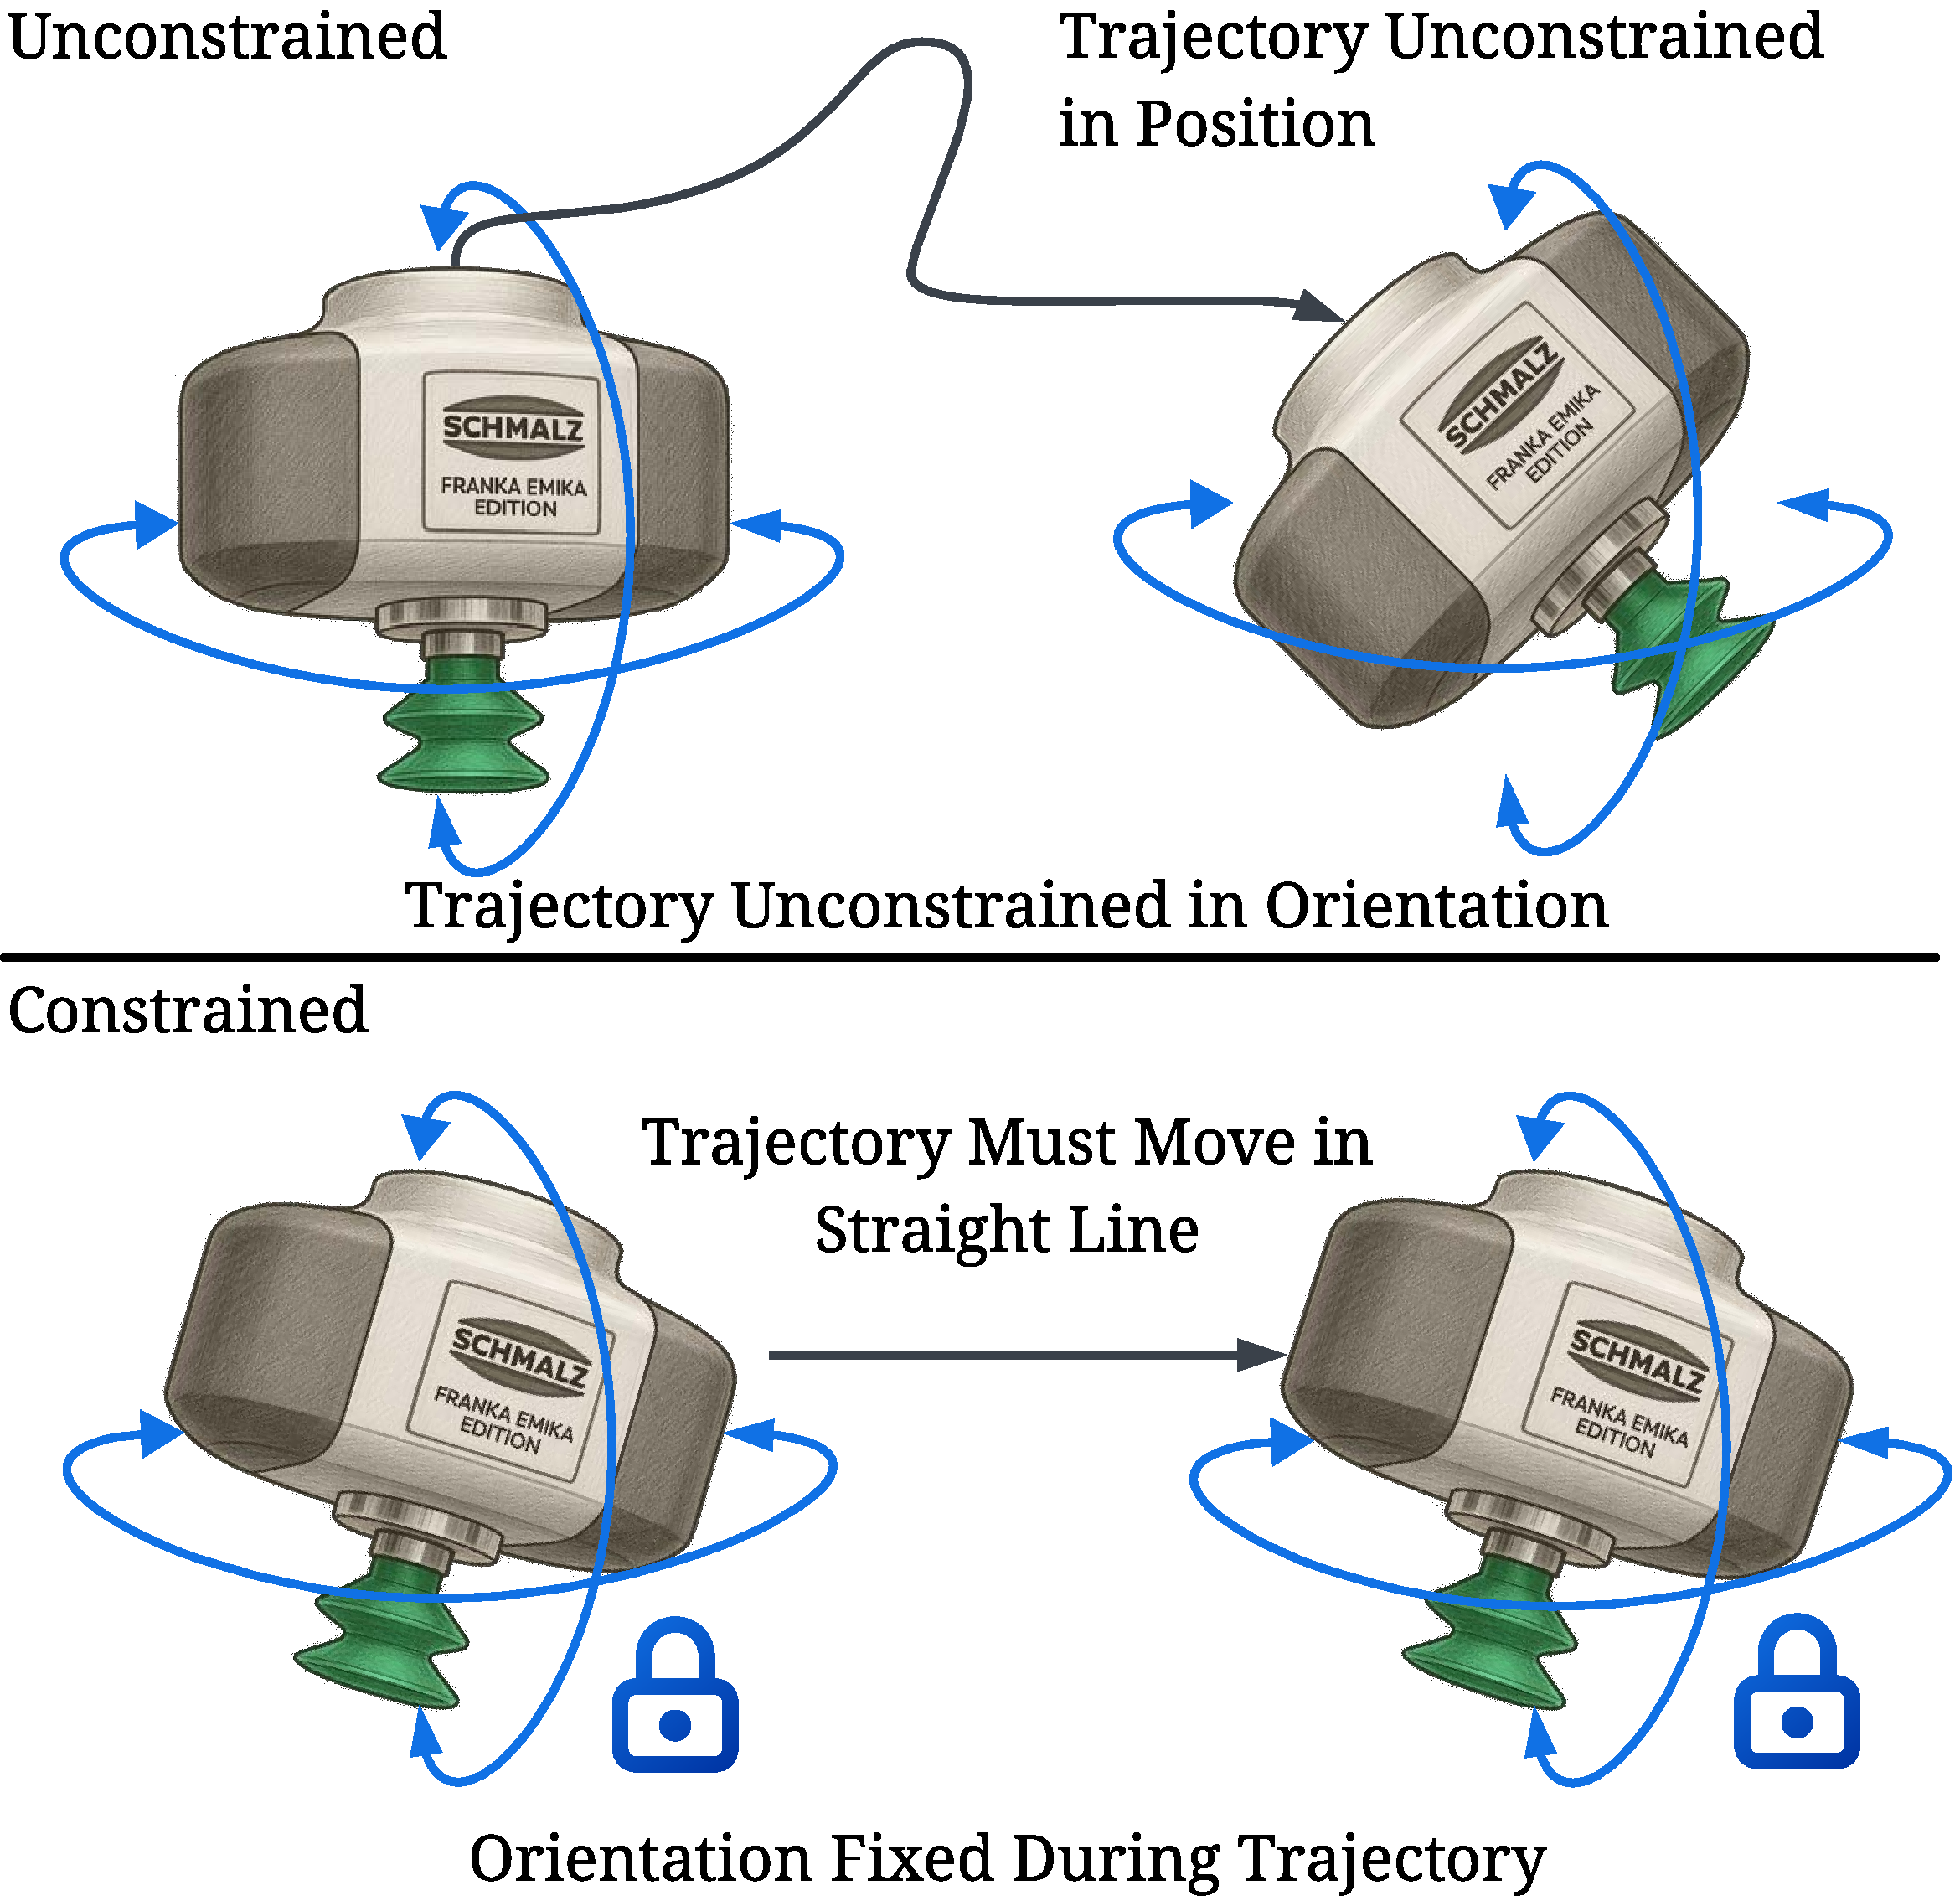
\includegraphics[width=0.9\columnwidth]{figures/primitives_explainer-compressed.pdf }
    \caption{Graphic description of the constraint definitions used in \cref{sec:sim-analysis}. The \texttt{unconstrained} primitive corresponds to a feasible trajectory between two points and includes unconstrained manipulation where the object is rigidly secured to the end-effector. The \texttt{constrained} corresponds to planar, approximately straight-line motion with minimal end-effector orientation change. \vspace{-25pt}}
    \label{fig:primitive-explain}
\end{figure}

\paragraph{Constraint Definitions}
Constraints correspond to task-relevant motion primitives. Unconstrained motion (\cref{fig:primitive-explain}, top) corresponds to a feasible trajectory between two points and includes manipulation primitives where the object is rigidly secured to the end-effector. The objective is to move from $\mathbf{q}_\text{s}\in\mathbb{R}^N$ to $\mathbf{q}_\text{g}\in\mathbb{R}^N$ with no additional geometric constraints beyond feasibility under failures.%
{\setlength{\abovedisplayskip}{6pt}\setlength{\belowdisplayskip}{6pt}\setlength{\abovedisplayshortskip}{4pt}\setlength{\belowdisplayshortskip}{4pt}%
\begin{equation}\small
\begin{aligned}
  \mathcal{T}_\text{Unconstrained}=\Big\{\mathbf{q}_t \forall t\in\{1,\dots,T\}\ \Big|\ 
  & \mathbf{q}_1=\mathbf{q}_\text{s},\  \mathbf{q}_T=\mathbf{q}_\text{g},\ \\
  & \mathbf{q}_t\in \mathcal{C}_t(\mathbf{q},\xi)\Big\}.
\end{aligned}
\end{equation}}%

Constrained motion (\cref{fig:primitive-explain}, bottom) corresponds to planar, approximately straight-line motion with minimal end-effector orientation change. This provides a spatial constraint for motion primitives such as pushing, pulling, or surface tracing. Let $\mathbf{p}_t\in\mathbb{R}^3$ be the end-effector position, $\mathbf{R}_t\in SO(3)$ its orientation, and $\mathbf{R}_\text{s}$ the initial orientation. Let $\mathcal{P}\subset\mathbb{R}^3$ be the designated plane. A trajectory satisfies \texttt{constrained} if, for all $t$, it obeys: (1) $\mathbf{p}_t\in\mathcal{P}$, (2) $\Delta p_t=\texttt{proj}_{\mathcal{P}}(\mathbf{p}_t)\le \epsilon_p$, (3) $\Delta \mathrm{R}_t=\|\mathbf{R}_t-\mathbf{R}_\text{s}\|_F\le \epsilon_R$, and (4) $\mathbf{q}_t\in \mathcal{C}_t(\xi)$. The valid trajectory set is:%
{\setlength{\abovedisplayskip}{6pt}\setlength{\belowdisplayskip}{6pt}\setlength{\abovedisplayshortskip}{4pt}\setlength{\belowdisplayshortskip}{4pt}%
\begin{equation}\small
\begin{aligned}
  \mathcal{T}_\text{Constrained}
  = \Big\{\mathbf{q}_{t}\ \forall t\in\{1,\dots,T\}\ \Big|\ &
  \mathbf{p}_t\in\mathcal{P}\ \land\ \\ \Delta p_t\le \epsilon_p,
   \Delta \mathrm{R}_t\le \epsilon_R\ & \land\ \mathbf{q}_t\in \mathcal{C}_t(\mathbf{q},\xi)
  \Big\}.
\end{aligned}
\end{equation}}%

\paragraph{Evaluation Metrics}
We applied statistical methods to test whether DEFT outperforms baseline approaches. Because success rates are bounded between 0 and 1 and often vary in spread, we used nonparametric methods that do not assume normally distributed data. To compare DEFT with the baseline under each failure condition, we estimated the difference in success rates using bootstrapping; if the 95\% confidence interval does not include zero, DEFT is considered better. To compare performance across groups of conditions (e.g., in-distribution vs. out-of-distribution, task constraint, or failure type), we used the Mann–Whitney U test, which is robust to unequal variances and outliers. To reduce the risk of false positives when making many comparisons, we applied false discovery rate (FDR) correction. Finally, to assess the overall effect of planner choice, we used a \(\chi^2\)\ test to ask whether using DEFT significantly changes the odds of satisfying constraints across all tasks.
%Together, these choices provide distribution-robust inference with controlled error rates that map directly to decisions an engineer would make (e.g., which planner to deploy).




% \begin{tabular}{|c|c|c|c|c|}
% \hline
% % \multicolumn{2}{|c|}{} & \multicolumn{3}{c|}{\textbf{Top Header for Last 3 Columns}} \\ \hline
% \multicolumn{2}{|c|}{} & \textbf{Baseline} & \textbf{DEFT} & \textbf{95\% C.I. } \\ \hline
% \multirow{H1} & Angle Failure & 48.2\% & \textbf{84.3}\% & [35.3\%-37.0\%]  \\ \cline{2-5}
%                          & Velocity Failure & 32.5\% & \textbf{70.8}\% & [37.8\%-38.8\%] \\ \hline
% \multirow{H2} & Constrained & 30.93\% & \textbf{46.42}\% & [--7.70\%, 34.50\%] \\ \cline{2-5}
%                          & Unconstrained & 42.4\% & \textbf{99.58\%} & [34.62\%, 79.85\%] \\ \hline
% \multirow{H3} & ID & \cellcolor{black} & \textbf{78.33\% }& \cellcolor{black} \\ \cline{2-5}
%                          & OOD & \cellcolor{black} & \textbf{73.61\%} & \cellcolor{black} \\ \hline
% \end{tabular}
% \caption{Success rate of the Baseline methods and the DEFT method. The 95\% Confidence Interval is on the improvement of DEFT over the baseline.}
% \label{tab:performance}
% \end{table}
% \vspace{5}
\subsubsection{Results} \label{sec:sim-results}
In this section, we demonstrate that DEFT significantly outperforms traditional planning baselines across various failure conditions. DEFT achieves a 37.66 percentage point improvement in constraint satisfaction compared to classical methods. We also show that DEFT generalizes well to unseen failure conditions, maintaining near-parity performance across in-distribution and out-of-distribution failure conditions. Finally, DEFT excels at handling both constrained and unconstrained motion tasks, with substantial gains in success rates across diverse constraints.
% We show within this setup, DEFT decisively outperforms classical baselines on all three hypotheses. \gm{add a teaser on what we show}



\paragraph{\textbf{H.1} Analysis}%
To evaluate whether DEFT produces trajectories that satisfy failure constraints at a higher rate than traditional planning baselines, we compare overall constraint satisfaction. DEFT achieves a success rate of 74.51\%, while the baseline achieves only 36.85\%. This represents an absolute improvement of 37.66 percentage points. A bootstrap analysis confirms the reliability of this difference ($p < 10^{-10}$), yielding a 95\% confidence interval of [37.21\%, 38.10\%] on the improvement in success rate. The specific performance rates for both angle and velocity failures can be seen in \cref{tab:performance}. Because the improvement holds across heterogeneous failure types and a wide range of sampled magnitudes, it indicates that DEFT generalizes to arbitrary joint-level degradations by conditioning directly on the failure embedding. In practice, given a new failure specification, DEFT translates it into feasible motion plans at substantially higher rates than the baseline.
 \vspace{-5pt}
% Further, we see significant improvments for angle and velocity failures for DEFT over the respective baselines, 84.3\% success rate for DEFT 48.2\% for the baseline in angle failure 
% The Mann-Whitney U with FDR correction for angle and velocity failures is  

\begin{table}[h]
\centering
\begin{tabular}{|c|c|c|c|}
\hline
\textbf{Hypothesis Summary} & \textbf{Test Condition}  & \textbf{Baseline} & \textbf{DEFT} \\ \hline
\textbf{H.1} Does DEFT handle & Angle Failure & 48.2\% & \textbf{84.3}\% \\ \cline{2-4}
arbitrary joint failures?& Velocity Failure & 32.5\% & \textbf{70.8}\% \\ \hline
\textbf{H.2} How well does DEFT & In Domain & \cellcolor{black} & \textbf{78.33\%} \\ \cline{2-4}
 handle unseen failures?& Out of Domain & \cellcolor{black} & \textbf{73.61\%} \\ \hline
\textbf{H.3} How well does DEFT  & Constrained & 30.93\% & \textbf{46.42}\% \\ \cline{2-4}
create multiple primitives?  & Unconstrained & 42.4\% & \textbf{99.58\%} \\ \hline

\end{tabular}
\caption{Success rate of the Baseline methods and the DEFT method. \vspace{-10pt}}
\label{tab:performance}
\end{table}

%   failure_type   deft_n  base_n  p_value  deft_success_rate  base_success_rate  significant  p_fdr
% 0        angle  1290400   13376      0.0           0.843308           0.482057         True    0.0
% 1     velocity  3417920   34822      0.0           0.707975           0.324852         True    0.0


\paragraph{\textbf{H.2} Analysis}
To test whether DEFT generalizes to unseen embodiment failure conditions, we tested success rates across in-distribution (ID) versus out-of-distribution (OOD) embodiment failure conditions, classified using Mahalanobis distance and k-NN distances in joint space. DEFT maintained a high constraint satisfaction rate as shown in \cref{tab:performance}. The small difference between ID and OOD performance indicates robustness to distributional shift. 
% In contrast, the baseline planner's OOD success rate was substantially lower (\textbf{37.70\%}).
Near-parity between ID and OOD success 
%, and the fact that even for failure conditions furthest from the training distribution (highest Mahalanobis-distance quartile) DEFT attains 68\% success,
indicates DEFT extrapolates over joint space rather than memorizing seen cases. Consequently, previously unseen failure configurations, regardless of which joint is affected or the magnitude of degradation, are translated into geometrically feasible, constraint-satisfying trajectories, evidencing DEFT’s ability to handle arbitrary failure conditions.



\paragraph{\textbf{H.3} Analysis}%
To assess whether DEFT more reliably satisfies task motion constraints, we evaluate performance separately for \texttt{unconstrained} (where the end effector can move freely, such as pick-and-place) and \texttt{constrained} (where the end effector must remain level and move in a straight line, such as surface tracing, pushing, and pulling) motions. The constraint satisfaction rate for both the categories as compared to the baselines (\cref{tab:performance}) shows that DEFT performs better for both primitives.
In the \texttt{unconstrained} setting, DEFT achieves a constraint satisfaction rate of 99.58\%, compared to 42.40\% for the RRT baseline, an absolute improvement of 57.18 percentage points. 
A Mann--Whitney U test on the \texttt{unconstrained} primitive difference between baseline and DEFT confirms that DEFT is statistically significant in 95.24\% of tested conditions after FDR correction, with a median bootstrap 95\% confidence interval on the improvement in success rate of [34.62\%, 79.85\%]. 
For the \texttt{constrained} motions, DEFT achieves 46.42\% satisfaction compared to the baseline's 30.93\%. A chi-squared test confirms that primitive constraint satisfaction is significantly associated with planner choice for both \texttt{unconstrained} and \texttt{constrained} primitives (\(\chi^2\text{ test},\ p<10^{-10}\)) , providing strong empirical support for \textbf{H.3}. It is important to note that the overall low success rate arises from the combined constraints of the primitive and the failure condition. For this evaluation, when excluding conditions, we checked only whether the randomly sampled start and goal satisfied the \texttt{constrained} constraints. However, this check does not guarantee that any feasible action exists, which likely contributes to the sub-50\% success rate.

These findings indicate that \textsc{DEFT} is not specialized to a single manipulation mode: it reliably synthesizes feasible trajectories for both \texttt{unconstrained} and \texttt{constrained} motions under the policy. 

\noindent\emph{Ablation note.} In simulation, conditioning yields similar constraint-obedience to an unconditioned diffusion ablation (within \(\approx\)1–2 percentage points overall), while delivering large gains in real-world task success (\cref{sec:real_world}).
 \vspace{-5pt}


\subsection{Real World}\label{sec:real_world}




Having established in simulation that \textsc{DEFT} generalizes to unseen failures and and reliably instantiates both \texttt{unconstrained} and \texttt{constrained} motions, we now test whether these gains translate to end-to-end task success on hardware. The next subsection evaluates \textsc{DEFT}, the hybrid RRT--Differential-IK optimization approach used in data generation (\cref{sec:data_generation}), and an ablation of DEFT without the conditioning input, \textsc{DEFT}-NoConditioning,  on two long-horizon, multi-primitive tasks (drawer and erasing). \vspace{-15pt}

% \begin{table}[h]
% \centering
% \caption{Drawer configuration: applied joint limits (rad).}
% \label{tab:limits_drawer}
% \setlength{\tabcolsep}{5pt}\footnotesize
% \begin{tabular}{lrrl}
% \hline
% \textbf{Joint} & \textbf{Lower} & \textbf{Upper} & \textbf{Note} \\
% \hline
% $J_1$ & 0.049775 & 0.049775 & LOCKED \\
% $J_2$ & -1.762800 & 1.762800 & NORMAL \\
% $J_3$ & -2.897300 & 2.897300 & NORMAL \\
% $J_4$ & -2.470927 & -1.925254 & REDUCED \\
% $J_5$ & -2.897300 & 2.897300 & NORMAL \\
% $J_6$ & 1.195150 & 2.623850 & REDUCED \\
% $J_7$ & -2.897300 & 2.897300 & NORMAL \\
% \hline
% \end{tabular}
% \end{table}

% \begin{table}[h]
% \centering
% \caption{Eraser (Whiteboard) configuration: applied joint limits (rad).}
% \label{tab:limits_eraser}
% \setlength{\tabcolsep}{5pt}\footnotesize
% \begin{tabular}{lrrl}
% \hline
% \textbf{Joint} & \textbf{Lower} & \textbf{Upper} & \textbf{Note} \\
% \hline
% $J_1$ & 0.033067 & 1.027757 & REDUCED \\
% $J_2$ & -1.762800 & 1.762800 & NORMAL \\
% $J_3$ & -2.897300 & 2.897300 & NORMAL \\
% $J_4$ & -3.071800 & -0.069800 & NORMAL \\
% $J_5$ & -0.073072 & 0.956709 & REDUCED \\
% $J_6$ & 1.865146 & 2.958065 & REDUCED \\
% $J_7$ & -2.897300 & 2.897300 & NORMAL \\
% \hline
% \end{tabular}
% \end{table}

\begin{table}[h]
\centering
\caption{Applied joint limits (rad) for real-world configurations. \textbf{Bold} indicates a locked joint; \emph{italics} indicate reduced limits.}
\label{tab:limits_drawer_eraser}
\setlength{\tabcolsep}{6pt}\footnotesize
\begin{tabular}{lrr|rr}
\hline
\textbf{Joint} & \multicolumn{2}{c|}{\textbf{Drawer}} & \multicolumn{2}{c}{\textbf{Erasing}} \\
 & \textbf{Lower} & \textbf{Upper} & \textbf{Lower} & \textbf{Upper} \\
\hline
$J_1$ & \emph{-0.81} & \emph{0.17} & \emph{0.033} & \emph{1.028} \\
$J_2$ & \emph{0.10} & \emph{1.50} & -1.763 & 1.763 \\
$J_3$ & \emph{-0.90} & \emph{0.60} & -2.897 & 2.897 \\
$J_4$ & \emph{-2.60} & \emph{-1.30} & \textbf{-2.59} & \textbf{-2.59}\\
$J_5$ & \emph{-0.10} & \emph{1.70} & \emph{-0.073} & \emph{0.957} \\
$J_6$ & \emph{0.90} & \emph{2.50} & \emph{1.865} & \emph{2.958} \\
$J_7$ & \emph{-0.85} & \emph{1.60} & -2.897 & 2.897 \\
\hline
\end{tabular}
\end{table}
\vspace{-10pt}

\begin{figure}[hbtp]
\vspace{2mm}
  \centering
  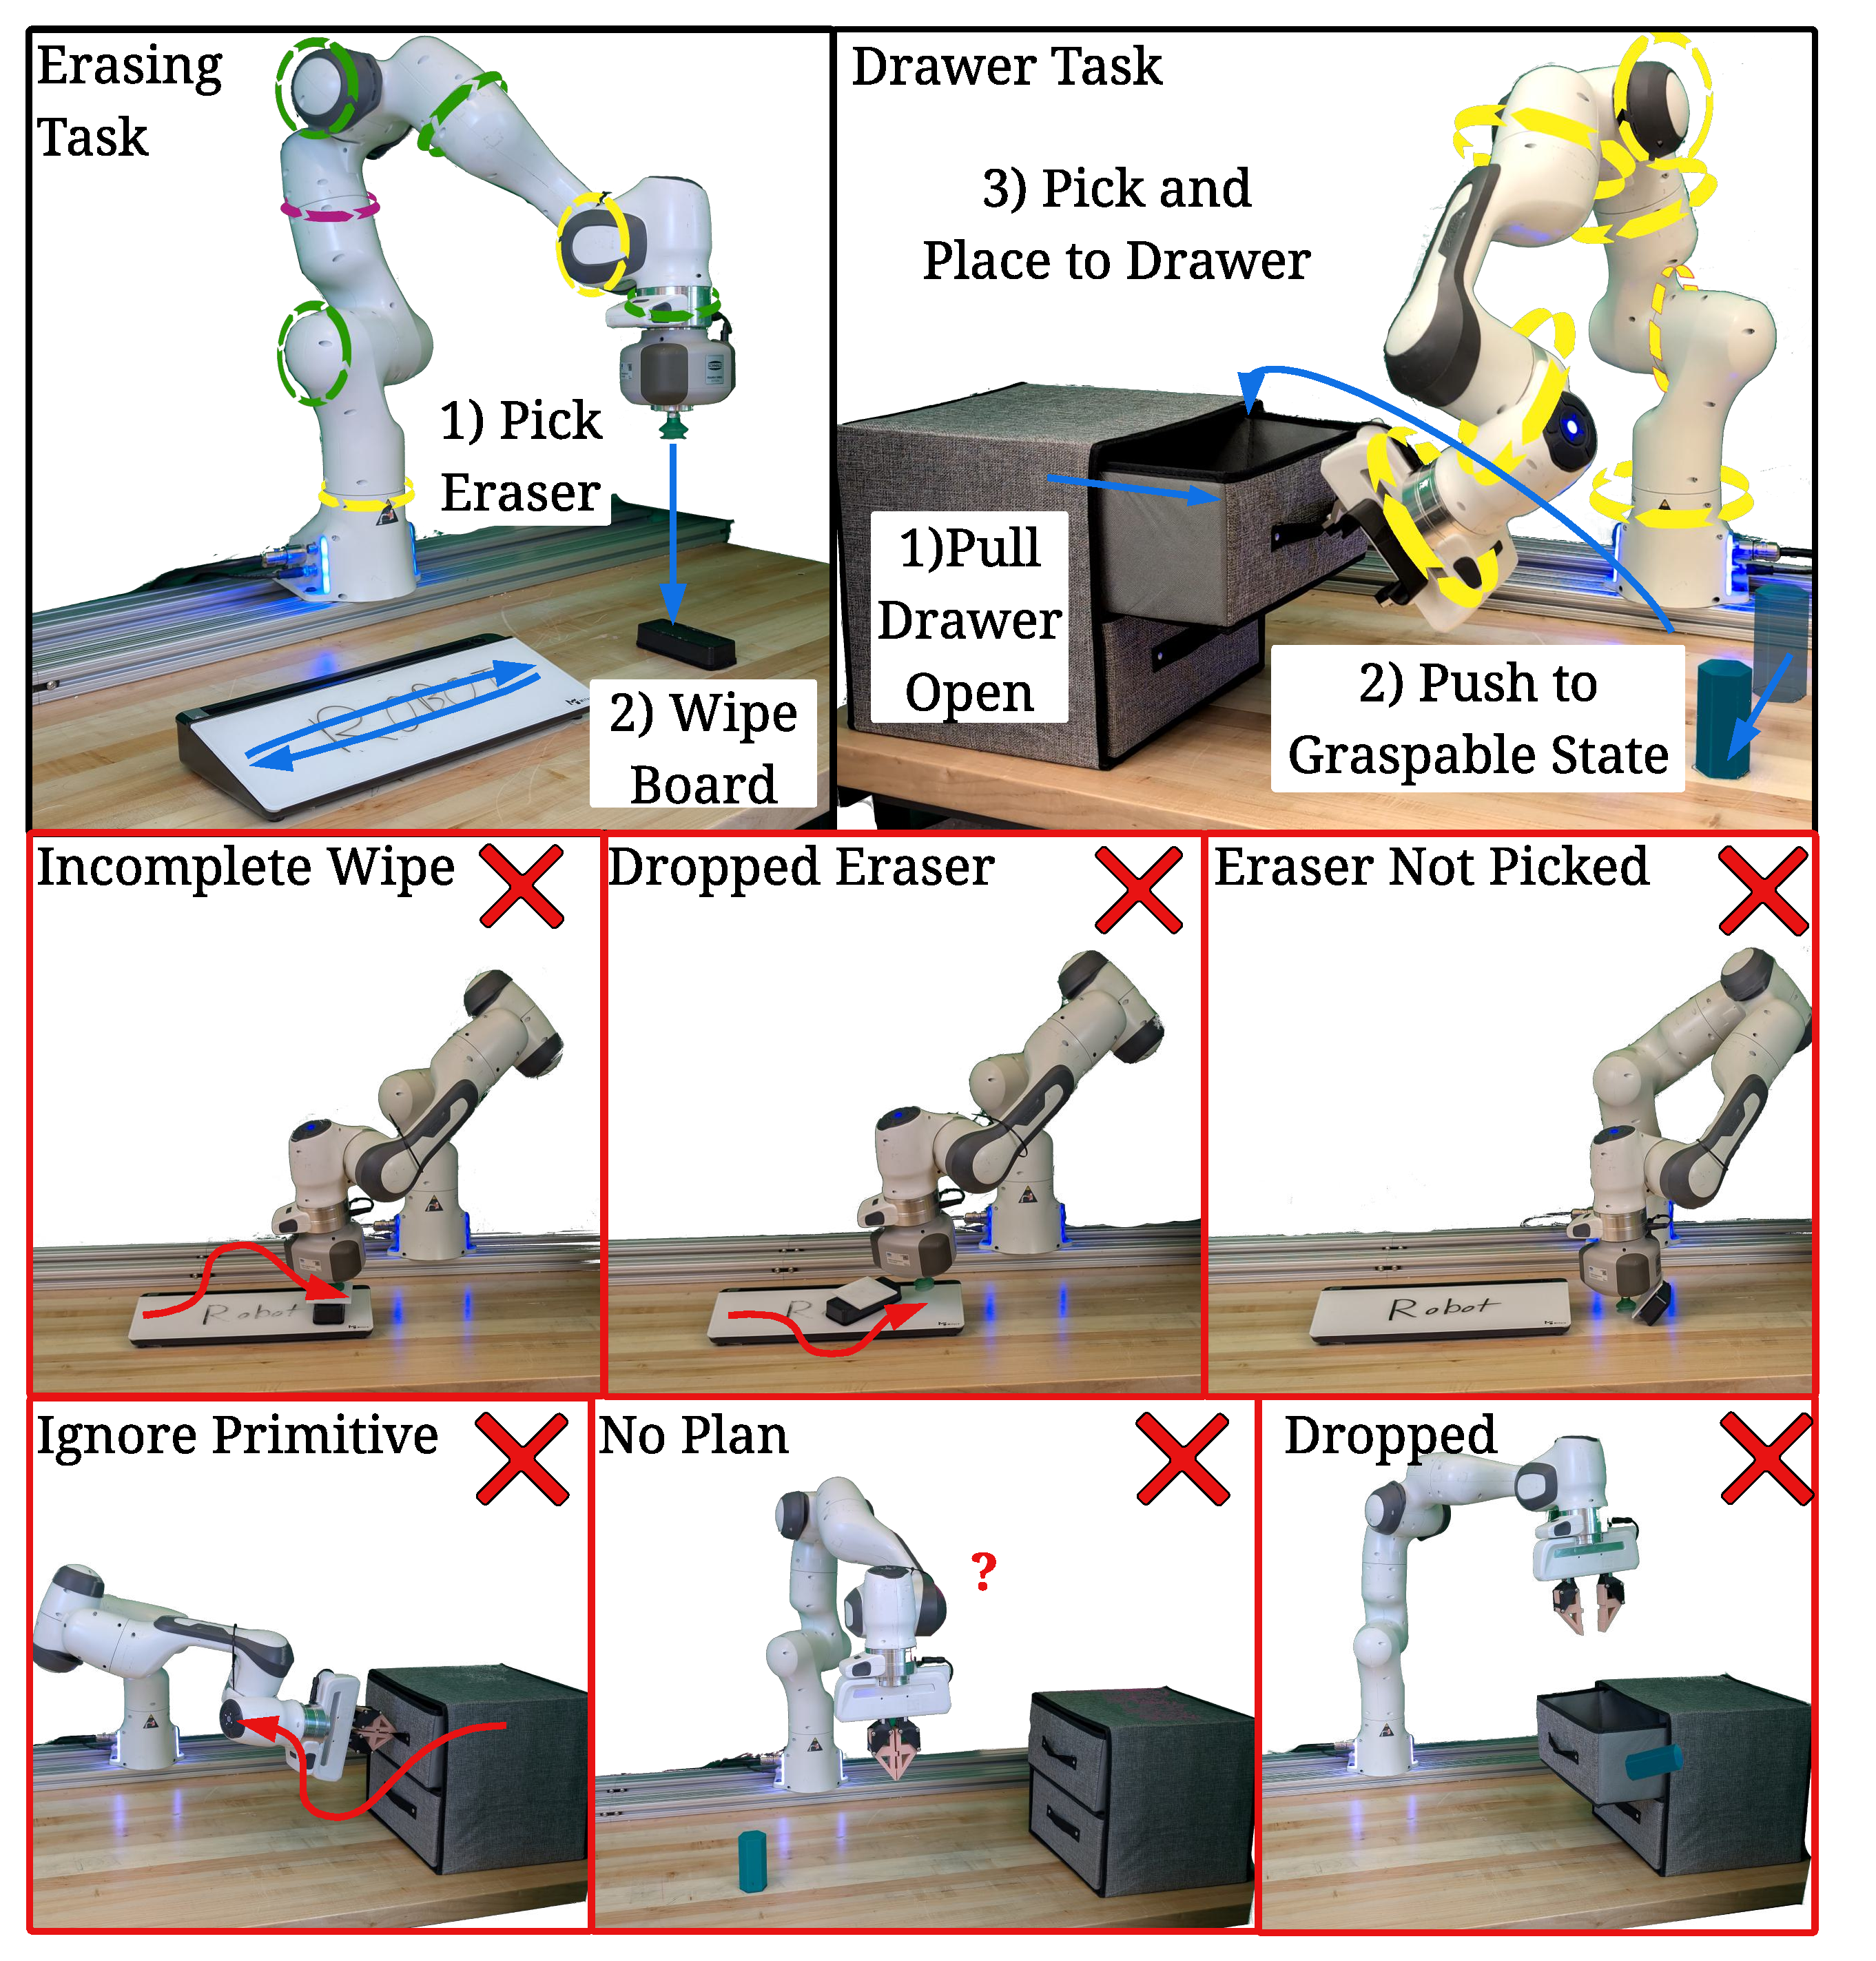
\includegraphics[width=\columnwidth]{figures/real-task-explainer-vertical-compressed-1.pdf}

  \caption{Left (Erasing): The robot grasps an eraser from the table and performs back-and-forth sweeps to remove text. Erasing failures include incomplete wipes or drops from disobeying motion constraints (improper normal force), and missed picks when lacking inpainting prevents reaching prescribed start/goal poses. Right (Drawer): The robot opens a drawer, pushes an object to a graspable pose, places it inside, and closes the drawer. Drawer failures include unopened drawers from ignored motion constraints, unfeasible plans under task constraints, and drops from unrespected target positions without inpainting.\vspace{-23pt}}
  \label{fig:real-world-tasks}
\end{figure}


\subsubsection{Task Description}  
We evaluate our system on two long-horizon, multi-step manipulation tasks that integrate both unconstrained and constrained actions, and that require transitions between unconstrained free-space motion and constrained contact-rich interaction. 

\paragraph{Drawer Task} (\cref{fig:real-world-tasks}, Top Right)
The drawer task consists of five sequential phases: (1) pulling the drawer open from its closed state, (2) pushing the object to a graspable position, (3) grasping an object from the workspace, (4) placing the object inside the drawer, and (5) pushing the drawer closed. The task combines unconstrained manipulation (picking and placing) with constrained manipulation (pushing and pulling), while alternating between unconstrained free-space motion and the constrained kinematics of the drawer. This structure creates distinct primitive requirements and embodiment sensitivities, making it effective for evaluating how conditioning and inpainting influence robustness. 

We assign scores of 1.0 for completing the task and 0.0 for not completing the task as all observed errors led to complete task failure. We evaluated 10 runs per approach.

\paragraph{Erasing Task}  
The erasing task requires the robot to first grasp an eraser from the table, then sweep it back and forth across a whiteboard to remove pre-written text. Here, unconstrained manipulation (picking) leads into constrained, contact-rich surface motion (erasing), requiring sustained alignment with the constrained geometry of the board. This task emphasizes embodiment-dependent failure recovery in a setting where continuous constraint satisfaction and primitive-specific control are necessary, providing a complementary evaluation to the drawer task. 

We partially score each trial up to 1.0 point: (i) +0.25 for picking the eraser, (ii) +0.50 for removing the target text with points awarded only for full removal of markings on the board, and (iii) +0.25 for retaining the eraser through the run. We evaluated 10 runs per approach.

\subsubsection{Failure Condition Description}
% For reproducibility, we list the joint limits enforced on the physical robot in \cref{tab:limits_drawer_eraser}. In the drawer task (\cref{fig:real-world-tasks}, right), locking $J_1$ removes base yaw, reducing the arm from seven to six degrees of freedom and eliminating a major redundancy axis. Narrowing the ranges of $J_4$ and $J_6$ restricts elbow and wrist motion, shrinking both the reachable and orientation workspaces, reducing null-space freedom, and lowering manipulability. In the erasing task (\cref{fig:real-world-tasks}, left), tightening $J_1$, $J_5$, and $J_6$ further limits global heading changes and wrist flexion/rotation, making orientation-constrained motions harder to realize.
For reproducibility, we list the joint limits enforced on the physical robot in \cref{tab:limits_drawer_eraser}. In the drawer task, all seven joints operate under reduced ranges. Collectively, these reductions shrink both reachable and orientation workspaces, diminish null-space freedom, and lower manipulability. In the erasing task, the elbow $J_4$ is locked at $-2.4$\,rad, removing one degree of freedom; $J_1$, $J_5$, and $J_6$ are reduced, further constraining end effector rotation and positioning.


\subsubsection{Results}
In the following section, we present real-world task results that further validate the findings from our simulations. \textsc{DEFT} consistently outperforms traditional baselines, achieving perfect task completion in both the Drawer and Erasing tasks. These results underscore the robustness of \textsc{DEFT} in handling joint-limit failures, showing how embodiment and primitive conditioning enable stable, feasible motion plans where optimization-based methods fail.
\vspace{-15pt}
\begin{table}[h]
\centering
\caption{Real-world task results over 10 runs. }
\label{tab:rw_tasks_combined}
\begingroup
\setlength{\tabcolsep}{5pt}
\renewcommand{\arraystretch}{1.1}
\footnotesize
\begin{tabular}{@{}llcc@{}}
\hline
\textbf{Model} & \textbf{Task} & \textbf{Mean} & \textbf{Std.}  \\
\hline
DEFT                & Drawer  & \textbf{1.00} & 0.00  \\
DEFT                & Erasing & \textbf{1.00} & 0.00 \\
Optimization        & Drawer  & 0.00 & 0.00 \\
Optimization        & Erasing & 0.35 & 0.32 \\
DEFT-NoConditioning & Drawer  & 0.60 & 0.49 \\
DEFT-NoConditioning & Erasing & 0.93 & 0.12 \\
\hline
\end{tabular}
\endgroup
\end{table}
\vspace{-11pt}
\paragraph{Drawer Task}
\textsc{DEFT} achieved perfect task completion on the drawer task (\cref{tab:rw_tasks_combined}). The Optimization baseline produced no executable plans. \textsc{DEFT}-NoConditioning succeeded in \(6/10\) runs. Qualitatively, Optimization repeatedly failed to find feasible trajectories in the constrained drawer setting. The unconditioned ablation failed for two reasons: 1) the lack of embodiment conditioning and 2) missing start--goal inpainting. These missing components caused surface-constraint violations and jerky motion leading to the robot dropping the object and being unable to open the drawer. \textsc{DEFT} alternated cleanly between unconstrained pick-and-place and constrained push and pulls without violating joint or contact limits.

\paragraph{Erasing Task}
\textsc{DEFT} again achieved perfect completion (\cref{tab:rw_tasks_combined}). The Optimization baseline had a success rate of 35\% and exhibited unstable surface interaction with poor contact maintenance. \textsc{DEFT}-NoConditioning had a success rate of 93\% but would disobey the contact constraints causing the robot to lose control of the eraser, consistent with missing embodiment conditioning and inpainting. Under a severe configuration (elbow locked at \(J_4=-2.4\,\mathrm{rad}\) with reduced wrist and base limits), \textsc{DEFT} maintained smooth, constraint-consistent sweeps while preserving grasp.

These outcomes support our central hypothesis: embodiment and task conditioning, coupled with inpainting and clamping, yield a policy that remains fail-active under embodiment degradation. 
Practically, they show that \textsc{DEFT} recovers performance in settings where traditional optimization either cannot plan or produces unstable motions, and where an unconditioned generative policy is brittle. 
Together with the simulation results, the real-world trials substantiate that a single conditioned diffusion policy sustains task success across multiple primitives and joint-limit failures. 
%Overall, we show that \textsc{DEFT} preserves functionality across failures through completing tasks that require continuous constraint satisfaction and behavior switching.


 % Across both tasks, \textsc{DEFT}’s embodiment- and primitive-aware conditioning (with joint-limit inpainting) yields reliable, constraint-compliant behavior: it achieves perfect completion and adherence to the intended motion primitive on every run. The optimization baseline struggles to discover robust contact sequences: in drawer closing it only achieved closure once (and did not reach perfect compliance), and in erasing it produced erratic, unstable contact with just one full success. The unconditioned diffusion policy (DEFT-NoConditioning) demonstrates strong task completion but systematically ignores the NPM constraint—scoring 0.75 on every drawer run and frequently dropping performance during contact-rich wiping—highlighting that conditioning and inpainting are not cosmetic, but necessary to enforce primitives and sustain reliable contact over long horizons. 



\section{Conclusion \& Future Work} 
One of the practical bottlenecks to long-horizon autonomy is surviving hardware faults without stopping. Building fail-active robots is necessary to maintain functionality under faults without constant human intervention. To that end, we presented \textit{DEFT}, a \textit{D}iffusion-based \textit{E}mbodiment-aware \textit{F}ail-active \textit{T}ask-conditioned trajectory generation framework that enables robots to adapt to joint failures while preserving task performance.
% By treating failure adaptation as conditional trajectory generation \emph{with diffusion}.
Without explicit replanning or policy switching, DEFT generalizes across multiple failure types and motion primitives. Experiments show DEFT maintains high success rates under multiple joint failures, especially in out-of-distribution scenarios. In real-world trials, DEFT executes reliably under previously unseen multi-joint failures, delivering high task success with strict joint limit compliance.
Future work will focus on real-time failure detection, cross-embodiment transfer to enable fail-active strategies learned on one robot architecture to generalize to different robot platforms, and expanding manipulation skills like pivoting or throwing. By reframing how robots respond to actuation failures, DEFT paves the way to the development of reliable autonomous systems capable of continuous operation under adverse conditions. 
\vspace{-10pt}
% \gm{add cross-embodiment}


% While many robotic systems offer remarkable manipulation capabilities, this mechanical complexity inherently multiplies the possibilities for component degradation and failure. This work proposes DEFT, a Diffusion-based Embodiment-aware Fail-active Task-conditioned trajectory generation framework that enables robots to adapt to arbitrary joint failures while maintaining task capabilities. By framing failure adaptation as a conditional trajectory generation problem and using diffusion models, our approach generalizes across diverse failure types and motion primitives without requiring explicit replanning or policy switching. Our experiments demonstrate DEFT's effectiveness over baseline methods, maintaining high success rates even with multiple simultaneous joint failures across both in-distribution and out-of-distribution conditions. Our future work will focus on developing an online adaptation method that can detect and respond to evolving failure conditions in real-time, rather than relying on predetermined failure states. We will also explore cross-embodiment transfer learning to enable fail-active strategies learned on one robot architecture to generalize to different robot platforms. Finally, we plan to incorporate additional manipulation capabilities such as pivoting or throwing which will further enhance the robot's ability to complete diverse tasks. By reframing how robots respond to mechanical failures, DEFT contributes to the development of reliable autonomous systems capable of continuous operation under adverse conditions. % 

\AtNextBibliography{\small}
\printbibliography
%===============================================================================

\clearpage
% The acknowledgments are automatically included only in the final and preprint versions of the paper.
% \acknowledgments{If a paper is accepted, the final camera-ready version will (and probably should) include acknowledgments. All acknowledgments go at the end of the paper, including thanks to reviewers who gave useful comments, to colleagues who contributed to the ideas, and to funding agencies and corporate sponsors that provided financial support.}

%===============================================================================

% no \bibliographystyle is required, since the corl style is automatically used.



% \input{sections/limitations}
% \input{sections/appendix}

\end{document}
